\documentclass[12pt,openany,twoside,a4paper,english,french,spanish,brazil]{abntex2}

\usepackage{cmap}	
\usepackage{lmodern}	
\usepackage[T1]{fontenc}	
\usepackage[utf8]{inputenc}		
\usepackage{lastpage}		
\usepackage{indentfirst}
\usepackage{color}	
\usepackage{graphicx}	
\usepackage{units}
\usepackage[brazilian,hyperpageref]{backref}
\usepackage[alf]{abntex2cite}
\usepackage{bold-extra}
\usepackage{eso-pic}

\renewcommand{\backrefpagesname}{Citado na(s) página(s):~}
\renewcommand{\backref}{}
\renewcommand*{\backrefalt}[4]{
	\ifcase #1 %
		Nenhuma citação no texto.%
	\or
		Citado na página #2.%
	\else
		Citado #1 vezes nas páginas #2.%
	\fi}%
% ---


\usepackage{fixos/customizacoes}
\usepackage{subfig}

% Dados pessoais
\autor{Gustavo Caltabiano Eichler}
\curso{Engenharia Eletrônica}

% Dados do trabalho
\titulo{Caracterização e Simulação de Amplificadores Valvulados}
\data{2019}
\palavraChaveUm{Modelagem}
\palavraChaveDois{Amplificadores Valvulados}

% Dados da orientacao
\orientador{Professor Doutor Daniel Chaves Café}
\coorientador{}

% Dados para a ficha catalográfica
\cdu{02:141:005.6}

% Dados da aprovação do trabalho
\dataDaAprovacao{01 de junho de 2013 -- Data da aprovação do trabalho}
\membroConvidadoUm{Titulação e Nome do Professor Convidado 01}
\membroConvidadoDois{Titulação e Nome do Professor Convidado 02}

% Dados pessoais
\autor{Gustavo Caltabiano Eichler}
\curso{Engenharia Eletrônica}

% Dados do trabalho
\titulo{Caracterização e Simulação de Amplificadores Valvulados}
\data{2019}
\palavraChaveUm{Modelagem}
\palavraChaveDois{Amplificadores Valvulados}

% Dados da orientacao
\orientador{Professor Doutor Daniel Chaves Café}
\coorientador{}

% Dados para a ficha catalográfica
\cdu{02:141:005.6}

% Dados da aprovação do trabalho
\dataDaAprovacao{01 de junho de 2013 -- Data da aprovação do trabalho}
\membroConvidadoUm{Titulação e Nome do Professor Convidado 01}
\membroConvidadoDois{Titulação e Nome do Professor Convidado 02}

\definecolor{blue}{RGB}{41,5,195}
\makeatletter
\hypersetup{
     	%pagebackref=true,
		pdftitle={\@title}, 
		pdfauthor={\@author},
    	pdfsubject={\imprimirpreambulo},
	    pdfcreator={LaTeX with abnTeX2},
		pdfkeywords={abnt}{latex}{abntex}{abntex2}{trabalho acadêmico}, 
		colorlinks=true,       		% false: boxed links; true: colored links
    	linkcolor=blue,          	% color of internal links
    	citecolor=blue,        		% color of links to bibliography
    	filecolor=magenta,      		% color of file links
		urlcolor=blue,
		bookmarksdepth=4
}
\makeatother
\setlength{\parindent}{1.3cm}
\setlength{\parskip}{0.2cm}  
\makeindex

\newcommand{\EqVolterra}{\begin{equation}
	y(t)=h_{0} + \sum_{n=1}^{N} \int_{a}^{b}\cdot\cdot\cdot\int_{a}^{b} h_{n}(\tau_{1},...,\tau_{n})\prod_{j=1}^{n}x(\tau - \tau_{j})d\tau1 \cdots d\tau_{n}
	\label{Equação de Volterra1}
	\end{equation}}
\newcommand{\integral}{\int_{-\infty}^{\infty}}

\newcommand{\FRFG}{Função de Resposta em Frequência Generalizada }
\newcommand{\kernels}{núcleos }
\usepackage{tikz}
\usetikzlibrary{arrows}
\usepackage{amsmath}
\usepackage{gensymb}

\begin{document}

\frenchspacing 
\imprimircapa
\imprimirfolhaderosto*

\begin{fichacatalografica}
	\vspace*{\fill}					% Posição vertical
	\hrule							% Linha horizontal
	\begin{center}					% Minipage Centralizado
	\begin{minipage}[c]{12.5cm}		% Largura
	
	\imprimirautor
	
	\hspace{0.5cm} \imprimirtitulo  / \imprimirautor. --
	\imprimirlocal, \imprimirdata-
	
	\hspace{0.5cm} \pageref{LastPage} p. : il. (algumas color.) ; 30 cm.\\
	
	\hspace{0.5cm} \imprimirorientadorRotulo~\imprimirorientador\\
	
	\hspace{0.5cm}
	\parbox[t]{\textwidth}{\imprimirtipotrabalho~--~\imprimirinstituicao,
	\imprimirdata.}\\
	
	\hspace{0.5cm}
		1. \imprimirpalavrachaveum.
		2. \imprimirpalavrachavedois.
		I. \imprimirorientador.
		II. Universidade de Brasília.
		III. Faculdade UnB Gama.
		IV. \imprimirtitulo\\ 			
	
	\hspace{8.75cm} CDU \nomecdu\\
	
	\end{minipage}
	\end{center}
	\hrule
\end{fichacatalografica}

\begin{folhadeaprovacao}

  \begin{center}
    {\ABNTEXchapterfont\large\imprimirautor}

    \vspace*{\fill}\vspace*{\fill}
    {\ABNTEXchapterfont\bfseries\Large\imprimirtitulo}
    \vspace*{\fill}
    
    \hspace{.45\textwidth}
    \begin{minipage}{.5\textwidth}
        \imprimirpreambulo
    \end{minipage}%
    \vspace*{\fill}
   \end{center}
    
   Trabalho aprovado. \imprimirlocal, \imprimirdatadaaprovacao:

   \assinatura{\textbf{\imprimirorientador} \\ Orientador} 
   \assinatura{\textbf{\imprimirmembroconvidadoum} \\ Convidado 1}
   \assinatura{\textbf{\imprimirmembroconvidadodois} \\ Convidado 2}
      
   \begin{center}
    \vspace*{0.5cm}
    {\large\imprimirlocal}
    \par
    {\large\imprimirdata}
    \vspace*{1cm}
  \end{center}
  
\end{folhadeaprovacao}

\begin{dedicatoria}
   \vspace*{\fill}
   \centering
   \noindent
	\textbf{Dedico este trabalho aos que presenciaram diariamente e acreditaram que com esforço, confiança e perseverança os objetivos possam ser alcançados sempre que se deseja. }

   \textit{} \vspace*{\fill}
\end{dedicatoria}

\begin{agradecimentos}
Agradeço primeiramente ao Prof. Dr. Daniel Chaves Café por todos as orientações, apoio, confiança e incentivos aos estudos e escrita deste trabalho.

Agradeço aos meus pais, José e Mônica, e minhas irmãs Bruna e Juliana por todo o apoio e confiança dados durante os estudos.

Agradeço a minha namorada, Luisa, por todo o apoio e suporte durante o período em que estive estudando. 

Agradeço à Universidade de Brasília e todos os professores por proporcionar todo o conhecimento e educação necessária para a formação deste trabalho.

\end{agradecimentos}

\begin{epigrafe}
    \vspace*{\fill}
	
\end{epigrafe}

\begin{resumo}

 O trabalho desenvolvido consistiu em utilizar as séries de Volterra como principal técnica para modelagem de sistemas não lineares. A criação de sinais capazes de extrair os parâmetros necessários para modelar um amplificador valvulado por meio da aplicação direta do modelo de \textit{Hammerstein}. Amplificadores valvulados são componentes fundamentais na amplificação de áudio, as características físicas de uma válvula modificam ligeiramente os sons amplificados resultando em timbres com características e nuances que se sobressaem em relação aos timbres obtidos com a utilização de amplificadores transistorizados. Os sons desses equipamentos é moldado tanto por suas características elétricas, como os filtros utilizados, tipos de válvula, capacitores, como por sua construção física, como tamanho da caixa e dos alto falantes. O objetivo deste trabalho é reproduzir as mesmas características elétricas, como a não linearidade do sistema.
 
 Complementando o trabalho anterior que contemplou a comparação de técnicas de modelagem com uma abordagem teórica para cada técnica citada, o desenvolvimento de uma metodologia para extrair os parâmetros não lineares, este trabalho tem como objetivo específico a criação de um modelo e a comparação com o sistema real modelado.

 \vspace{\onelineskip}
    
 \noindent
 \textbf{Palavras-chaves}: Modelagem, Amplificadores Valvulados, Séries de Volterra.
\end{resumo}

\begin{resumo}[Abstract]
 \begin{otherlanguage*}{english}
 This work consists of modelling non-linear systems through the use of Volterra Series and the creation of signals to extract the kernels of Volterra Series from the device under test to apply in a Hammerstein Model. Tube guitar amps has unique characteristics on processing sounds that differentiate from the sound of transistorized amps. The main objective of this work is to reproduce these unique characterists in an virtual model.
 
 Complementing a previous work in comparing different techniques of non-linear modelling, a methodology was developed to build a virtual model and compare to the real tube amp.
   \vspace{\onelineskip}
 
   \noindent 
   \textbf{Key-words}: Tube amps, Volterra Series, Non-linear modelling.
 \end{otherlanguage*}
\end{resumo}

\pdfbookmark[0]{\listfigurename}{lof}
\listoffigures*
\cleardoublepage
\pdfbookmark[0]{\listtablename}{lot}
\listoftables*
\cleardoublepage

\pdfbookmark[0]{\contentsname}{toc}
\tableofcontents*
\cleardoublepage


\textual

\chapter[Introdução]{Introdução}


A engenharia envolvida por trás da música sempre foi um assunto presente e causador de grandes mudanças. Seguindo uma tendência muito forte nos dias atuais, a engenharia modernizou o mundo da música tirando-a de um mundo analógico e introduzindo ao cenário digital, não só o modo como escutamos as músicas passou a ser digital, mas também o modo como se toca os instrumentos. Em 1996, a modelagem digital de amplificadores valvulados ganhou vida com o lançamento de um amplificador produzido pela \textit{Line 6}, uma empresa americana de instrumentos e acessórios para guitarra. Pela primeira vez na história, um amplificador utilizava um software embarcado em um chip \textit{DSP} (chip digital dedicado para processamento de sinais) como principal componente para modificar o som e os parâmetros de um amplificador \cite{paulwhite_line6_line6_line6_2006}. O \textit{Axsys 212}, mostrado na figura \ref{fig1}, como era chamado, foi um amplificador pioneiro que abriu uma gama de estudos e pesquisas na área de processamento de sinais de áudio.

\begin{figure}
	\centering
	\subfloat[]{
		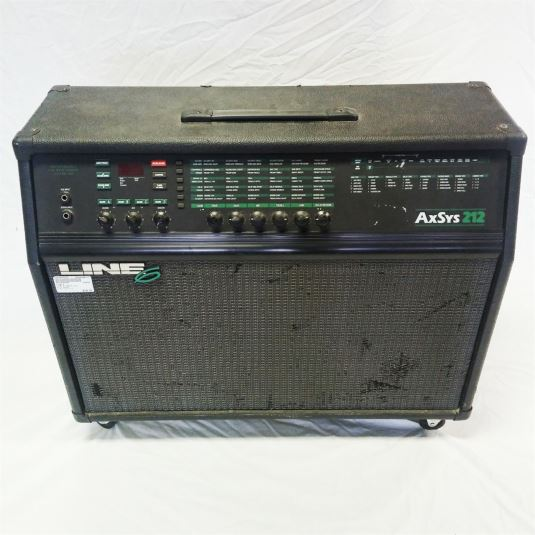
\includegraphics[height=5cm]{figuras/Axsys212}
		\label{fig:darthvader}
	}
	\subfloat[]{
		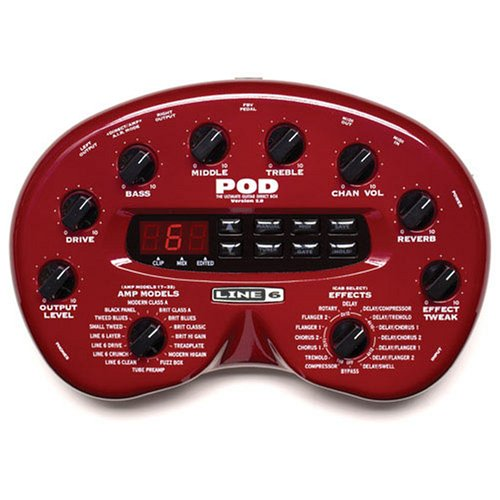
\includegraphics[height=5cm]{figuras/Pod}
		\label{fig:yoda}
	}
	\caption{(a): Line 6 Axsys 212. (b): Line 6 Pod }
	\label{fig1}
\end{figure}



Apesar de toda a inovação, a grande revolução na modelagem de amplificadores começou a ser feita dois anos após o lançamento do \textit{Axsys 212}, com a criação de um simulador portátil de amplificadores, o \textit{POD}, também da \textit{Line 6}, mostrado na figura \ref{fig1}. A qualidade das simulações de amplificadores valvulados na época aumentou consideravelmente e passaram a ser utilizadas para a realização de gravações em estúdios profissionais, onde a qualidade de som é um parâmetro essencial. O uso desses simuladores ganhou grande visibilidade e espaço entre os amplificadores analógicos pelo fato de ser um dispositivo portátil, leve e com uma variedade enorme de timbres, uma vez que um único simulador contém dezenas de modelos de amplificadores diferentes. A modelagem de amplificadores busca extrair todas as características de um amplificador valvulado que personalizam o som produzido pela guitarra. 



As válvulas foram muito utilizadas em amplificadores até a invenção dos transistores que tomaram conta da maioria dos amplificadores produzidos atualmente, porém músicos experientes e treinados são capazes de perceber diferenças entre os sons produzidos por amplificadores valvulados e transistorizados. Alguns estudos evidenciam a preferência dos músicos pelos valvulados, onde a diferença predominante para os amplificadores transistorizados é a resposta em frequência de sinais com alta intensidade, ou seja, como amplificador modifica sons graves e agudos \cite{bussey1981tubes}. 

A modelagem desses amplificadores busca caracterizar, com a maior fidelidade possível, o modo como as válvulas tratam sinais de áudio. Como a saturação, ou distorção, gerada pelas válvulas é muito mais suave do que as distorções geradas por transistores, os amplificadores valvulados tendem a ter um som mais agradável ao ouvido humano. 

Os amplificadores valvulados, basicamente, são compostos por:

\tikzstyle{int}=[draw, fill=blue!20, minimum size=2em]
\tikzstyle{init} = [pin edge={to-,thin,black}]
\begin{figure}	[!htb]
	\centering
	
	
	\begin{tikzpicture}[node distance=4cm,auto,>=latex']
	
	\node (a) {Pré};
	\node (b)  {a};
	
	\node [int] (a) {Pré Amplificador};
	\node [int] (c) [right of=a] {Equalização};
	\node [int] (d) [right of=c,node distance=4.5cm] {Amplificador de Potência};
	\node (b) [left of=a,node distance=4cm, coordinate] {a};
	\node [coordinate] (end) [right of=d, node distance=4cm]{};
	\path[->] (b) edge node {Entrada} (a);
	\path[->] (a) edge node {} (c);
	\path[->] (c) edge node {} (d);
	\draw[->] (d) edge node {Saída} (end) ;
	
	
	\end{tikzpicture}
	\caption{Principais componentes de um amplificador de guitarra}
	\label{Diagrama01}
\end{figure}

\begin{itemize}
	\item Pré amplificação: é o primeiro estágio de amplificação onde ocorre a primeira saturação, ou seja o primeiro estágio não linear, geralmente composto por válvulas do tipo triodo e um controle de volume;
	\item Equalização: Parte linear encarregada de filtrar o sinal, geralmente é divida em 3 bandas, sendo essas, graves, médios e agudos;
	\item Potência:é responsável por mais um estágio de amplificação, geralmente composto de pentodos, onde a saturação ocorre devido a uma forte não linearidade presente nas válvulas;
\end{itemize}

A modelagem de cada um dos estágios mostrados na figura \ref{Diagrama01} pode ser separada em duas classes:

\begin{itemize}
	\item Sistemas Lineares: Equalização;
	\item Sistemas Não Lineares: Pré amplificação e Amplificação de potência; 
\end{itemize}


A modelagem de amplificadores pode ser baseada então em algumas categorias como: aproximação por caixa preta (\textit{black box approach}), análise de todos os componentes discretizados (\textit{white box approach}), função de transferência linear e não linear entre muitas outras que podem ser vistas com mais detalhes em \cite{pakarinen2009review}.

Além da modelagem digital é possível também modelar amplificadores de forma analógica. Em 199,3 a empresa Tech 21, lançou um pedal de guitarra (SansAmp GT2) que incorporava as características do som de um amplificador valvulado, como a incorporação de harmônicos e distorções simétricas causadas pelas válvulas. Com uma operação muito simples o SansAmp GT2, mostrado na figura \ref{fig:sansamp}, possui três modelos de amplificadores diferentes, cada um desses amplificadores modelados foram baseados em amplificadores famosos sendo eles: Mesa/Boogie para o California, Marshall para o \textit{British} e Fender para o \textit{Tweed}. Cada um dos amplificadores possui três opções de timbre, com a chave MOD, é possível escolher três modos que modificam a distorção do sinal. Também existe a opção de alterar a emulação da posição do microfone que supostamente estaria captando o som do amplificador. Além dessas opções o pedal conta com um controle de volume, um equalizador de duas bandas e um ajuste de ganho.
\begin{figure}[!htb]
	\centering
	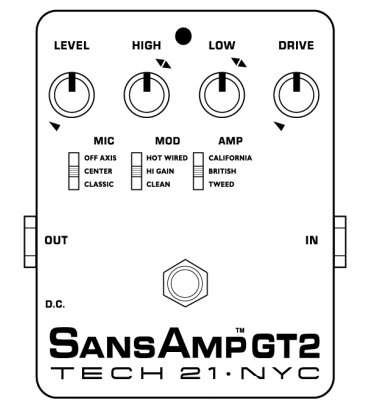
\includegraphics[width=0.7\linewidth]{figuras/SanSamp}
	\caption{SansAmp GT2 .Fonte: Manual do Usuário do SansAmp GT2}
	\label{fig:sansamp}
\end{figure}



\section*{O problema a ser abordado}
Os amplificadores de guitarra sempre foram um dos principais elementos entre todos os equipamentos necessários para um guitarrista. É indispensável para um som de qualidade, um amplificador que possua bons timbres e, na história dos amplificadores existem modelos que ficaram consagrados por timbres únicos e diferenciados. Até pouco tempo atrás, para se reproduzir o som de um amplificador de época - como são chamados os modelos com timbres diferenciados - era necessário possuir o amplificador em questão. O surgimento de técnicas de processamento digital de sinais permitiu reproduzir características desses amplificadores em dispositivos pequenos e portáteis, possibilitando assim, uma grande variedade de modelos de amplificadores famosos sem o problema de ter que se possuir os modelos físicos. Desde a sua criação, a modelagem digital de amplificadores valvulados vem se reinventando desde a sua criação. Sempre inovando na forma com que os amplificadores são modelados e na qualidade do som. O surgimento do \textit{Kemper Profiling Amp}, em 2013, mostrado na figura \ref{fig:profilingampbk-large}, trouxe uma nova visão ao mundo da modelagem de amplificadores. Este dispositivo realiza, em tempo real, a emulação de amplificadores valvulados através do método de caixa preta, ou seja, sem conhecer o circuito do amplificador e nem quais componentes constituem o amplificador \cite{kemper2014musical}.

\begin{figure}[!htb]
	\centering
	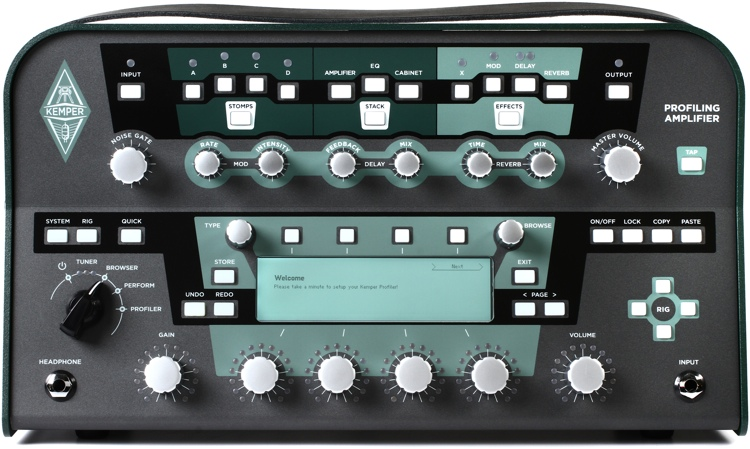
\includegraphics[width=0.7\linewidth]{figuras/ProfilingAmpBK-large}
	\caption{Amplificador Kemper Profiling Amp}
	\label{fig:profilingampbk-large}
\end{figure}




O \textit{Kemper} é capaz de modelar qualquer amplificador de guitarra de forma automática. Através da aplicação e gravação de sinais de teste, cria-se um modelo com características que imitam um amplificador real e salva em sua memória permitindo ao usuário utilizar o modelo posteriormente. 

A modelagem feita por esse amplificador depende então de se possuir o amplificador de referência para que os sinais possam ser aplicados e o amplificador então pode gerar o modelo digitalizado do amplificador. Para contornar o problema de ter que possuir todos os amplificadores que se deseja modelar, é possível inserir modelos já prontos através do compartilhamento de arquivos via Internet. Uma pessoa que já tenha realizado uma modelagem de um amplificador qualquer, pode disponibilizar para todos os usuários do \textit{Kemper} um arquivo que contém um certo amplificador modelado, com isso é possível inserir vários modelos no amplificador.

O \textit{Kemper}, faz uso de técnicas que modelam apenas como o amplificador modifica e distorce o som, ou seja, são técnicas que relacionam o sinal de entrada do amplificador com a saída, independente da forma e dos componentes eletrônicos utilizados na construção do amplificador a ser modelado. De forma semelhante, este trabalho busca modelar amplificadores através de técnicas que permitam criar modelos através de uma relação da entrada e saída de um amplificador real.

As séries de Volterra, criada por Vito Volterra em 1930, é uma das primeiras de caracterização sistemática de sistemas não lineares, essencialmente é uma extensão da convolução de sistemas lineares para sistemas não lineares \cite{cheng2017volterra}. Como as válvulas que compõem os amplificadores são dispositivos não lineares, que funcionam através do efeito termoiônico, o modelo de \textit{Hammerstein} da série de Volterra é ideal para realizar a modelagem de um amplificador valvulado






\section*{Objetivos}
\subsection*{Objetivos Gerais}
O método e os sinais utilizados pelo \textit{Kemper} permanecem em segredo da empresa. Além disso as técnicas de modelagem como amplificadores são complexas e dependem de um conhecimento muito específico para serem aplicadas. Técnicas não paramétricas que poderiam ser utilizadas de forma automatizada, extraem os parâmetros lineares dos amplificadores. No entanto, a principal característica de um amplificador valvulado é a não linearidade do sistema e a consequente distorção gerada.

O estudo sobre séries de Volterra foi uma das formas encontradas para se analisar e caracterizar sistemas não lineares, como amplificadores valvulados. Essa série permite a realização de uma análise de sistemas não lineares por meio de coeficientes chamados núcleos da série de Volterra. Esses \kernels são respostas ao impulso do amplificador em análise e, apesar da sua difícil obtenção, podem ser obtidos através de diferentes formas que serão abordadas nos próximos capítulos.

Sabendo que a maior parte dos estudos de modelagem tem foco em 
características lineares dos amplificadores, este trabalho tenta melhorar a modelagem de amplificadores de áudio incluindo 
componentes não-lineares desses amplificadores. Nossa intensão é que essa modelagem se aproxime mais do som real 
dos amplificadores de época.

\subsection*{Objetivos Específicos}
\begin{itemize}
	\item Extrair os parâmetros necessários para a modelagem de um amplificador;
	\item Criar um modelo digital de um amplificador;
	\item Avaliar o desempenho do modelo criado.
\end{itemize}

Este trabalho é organizado como se segue. O capítulo 2 sumariza as técnicas de modelagem de amplificadores mais conhecidas, introduz a teoria necessária para a utilização das séries de Volterra e define a escolha do sinal para extrair as características de um amplificador

\chapter{Modelagem de sistemas não lineares}

A modelagem de sistemas não lineares pode ser feita de diversas formas, cada uma com vantagens e desvantagens próprias. As técnicas de modelagem não linear mais relevantes serão revisadas a seguir, apresentando um panorama geral de como elas funcionam e como são aplicadas.

\section*{\textit{Static Wave Shaping}}
\textit{Static Wave Shaping} significa modelagem estática de ondas. Esta técnica é consiste em aplicar um mapeamento da não linearidade do sistema relacionando a variável de entrada com uma variável de saída. A implementação dessa técnica se dá pela modelagem de equações que representam a não linearidade, como por exemplo:
\begin{equation}
y = \frac{3x}{2} (1 - \frac{{x^2}}{3})
\label{Equação1}
\end{equation}
Essa equação proposta por \cite{arayasuyama}  é implementada para se obter distorção de um sinal. A distorção se dá pela alimentação do sinal, que tem sua amplitude normalizada entre -1 e 1, na equação não linear através dos coeficientes de escala \cite{pakarinen2009review}. A função mostrada acima é descrita na imagem \ref{fig:staticwaveshaping}, onde ela apresenta uma certa linearidade para sinais pequenos de entrada e uma parte não linear quando se aproxima dos limites de x, entre -1 e 1.
\begin{figure}[htb!]
	\centering
	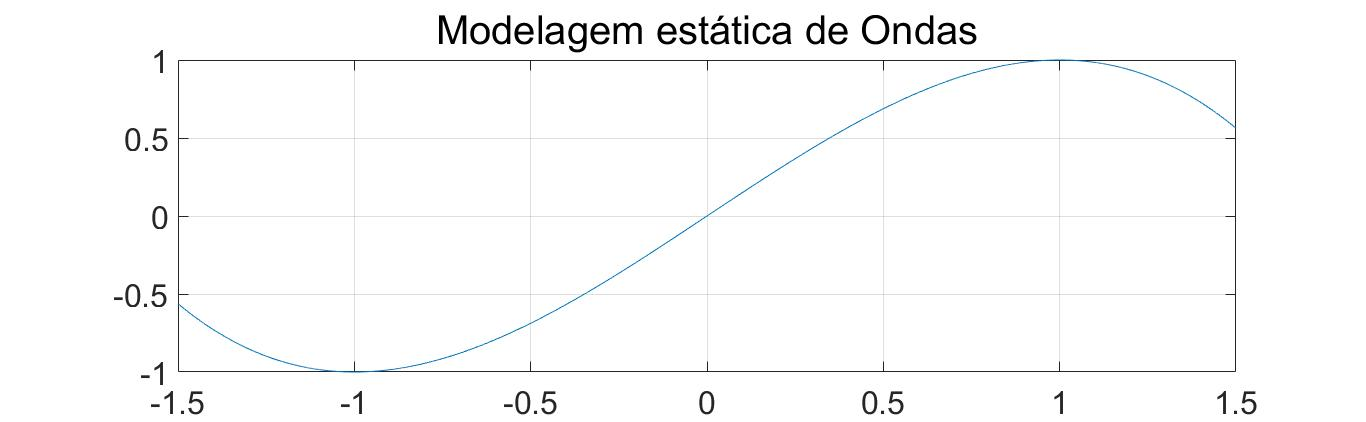
\includegraphics[width=0.7\linewidth]{figuras/StaticWaveShaping}
	\caption{Função não linear proposta por Araya e Suyama}
	\label{fig:staticwaveshaping}
\end{figure}

Um outro estudo realizado por \cite{moller2002measurement} apresenta um algorítimo para medir funções de transferências não lineares através de simulações utilizando o \textit{PSPICE}. O objetivo central do estudo era realizar uma mimica dos estágios de amplificação de um \textit{VOX AC 30}. Combinando simulações do esquemático elétrico do amplificador e exportando os dados obtidos para o \textit{MATLAB}.

\section*{\textit{Lookup Table Nonlinearity}}

A equação \ref{Equação1} pode ser também implementada através de uma técnica onde são pré computados os valores de saída para um valor determinado de entrada. A vantagem dessa técnica é a possibilidade de alterar os valores pré computados de maneira livre, sendo assim totalmente customizável\cite{pakarinen2009review}. A quantidade de dados que as tabelas contém está diretamente relacionada a resolução, ou seja, a qualidade e quantidade de detalhamento do som. Essa técnica foi utilizada pela Digidesign em um sintetizador que tinha como uma de suas funções, emular o som de uma guitarra distorcida. 

Estudos mais recentes realizados com \textit{Lookup Tables}
aproximam as tabelas com modelos \textit{Hammerstein}, que consistem em uma não linearidade estática, seguida por um filtro linear\cite{LUTFilter}. Esses modelos de \textit{Hammerstein} serão abordados mais detalhadamente posteriormente.

\section*{Análise nodal}
Através das Leis de Kirchhoff é possível obter o comportamento dos circuitos eletrônicos, utilizando modelos acurados dos componentes que compõem os amplificadores é possível relações aproximadas entre as tensões e as correntes que circulam pelo circuito \cite{pakarinen2009review}. Através de uma matriz de condutâncias, as tensões se relacionam com as correntes da seguinte forma:
\begin{equation}
Gv = \textit{c} 
\label{Equação2}
\end{equation}

Onde G na equação \ref{Equação2} é a matriz de condutâncias, \textit{v} é um vetor para cada voltagem no circuito e \textit{c} é o vetor que representa qualquer fonte de corrente em cada nó do circuito. Cada tipo de componente do circuito (resistor, capacitor, indutor, indutância mútua de transformadores,diodos, transistores) contribui com uma linha da matriz G. As correntes nas fontes de voltagem dependem de equações auxiliares que são adicionadas em colunas e linhas do sistema descrito acima. Esse método é chamado também de \textit{K-Method}, referindo-se as leis de Kirchhoff.
\begin{equation}
c=M_{1}x + M_{2}u + M_{3}i
\label{Equação3}
\end{equation}

Para aplicar o \textit{K-method}, a variável C na equação \ref{Equação2} é descrita pela equação \ref{Equação3}, onde é necessário escolher como as varáveis de estado \textbf{x}, as voltagens entre os capacitores e as correntes de indutores. A variável \textbf{u}, representa as fontes de corrente e voltagem presentes na entrada do circuito. Dispositivos não lineares contribuem com correntes não lineares \textbf{i} que são computadas por uma função vetorial \textbf{f} que mapeia as tensões controladas pelas correntes nos terminais dos dispositivos \cite{yeh2010automated1}. Como as correntes não lineares são dependentes das voltagens nos terminais de cada dispositivo não linear, a variável \textbf{i} é escrita em função de \textbf{v}. Então é possível modificar a equação \ref{Equação2} por:

\begin{equation}
Gv = M_{1}x + M_{2}u + M_{3}i(v) 
\label{Equação4}
\end{equation}

Essa técnica de modelagem, no entanto, depende da quantidade de nós que compõem o circuito para estimar o gasto computacional. Circuitos de amplificadores valvulados tendem a ser complexos e assim compromete a aplicação dessa técnica em tempo real.

\section*{\textit{Wave Digital Filters}}
\textit{Wave Digital Filters} são uma classe de filtros digitais onde é possível mapear seus parâmetros através das grandezas elétricas, como a tensão e a corrente. Cada elemento de um circuito elétrico possui uma representação em forma de filtro e através do uso de adaptadores é possível conectar diferentes filtros, como se fossem elementos de um circuito elétrico \cite{pakarinen2009review}. A construção de circuitos utilizando a técnica de \textit{Wave Digital Filters} se mostra eficiente e promissora para aplicações em tempo real, apesar de existirem algumas barreiras e topologias que não são mapeadas facilmente pela técnica.

O princípio por trás de \textit{Wave Digital Filters} é a transformação das variáveis de \textit{Kirchhoff}, tensão \textbf{v} e corrente \textbf{i}, em parâmetros utilizados na criação dos filtros, chamados de variáveis de onda (reflectância e incidência) \cite{2012Macak}.

A figura \ref{fig:componentesemwdf} resume as transformações para cada componente básico de um circuito.
\begin{figure}[!htb]
	\centering
	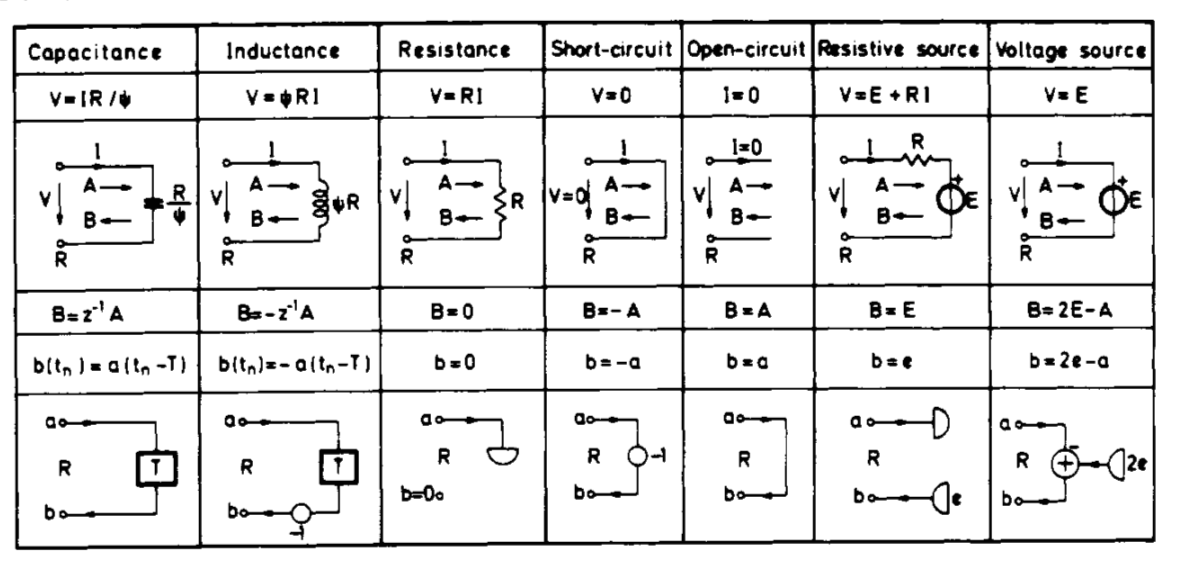
\includegraphics[width=0.7\linewidth]{figuras/ComponentesemWDF}
	\caption{Elementos básicos de um circuito e suas representações em grandezas de onda. Autor \cite{fettweis1986wave}.}
	\label{fig:componentesemwdf}
\end{figure}




\section*{Séries de Volterra}{\label{Volterra}}
É um método analítico que usa uma ferramenta matemática chamada séries de Volterra para modelar um sistema não linear. Série de Volterra é, por definição, uma convolução multidimensional da entrada do sistema com uma matriz de resposta não linear. Enquanto a resposta ao impulso em sistemas lineares caracteriza por completo um sistema e permite prever uma resposta para uma determinada entrada, em sistemas não lineares, esse tipo de caracterização não consegue identificar as não linearidades, caracterizando assim somente a parte linear do sistema. As Séries de Volterra permitem caracterizar, através de funções especiais, chamadas de \textit{kernels}, a parte não linear do sistema. Os \kernels correspondem a resposta multidimensional ao impulso dos coeficientes não lineares do sistema. \cite{pakarinen2009review}

As séries de Volterra podem ser consideradas também como uma expansão em séries de Taylor com os coeficientes do polinômio substituídos por convoluções multidimensionais representando assim o efeito de memória de sistemas não lineares de acordo com a ordem de não linearidade \cite{pakarinen2009review}



\subsection*{Definição no domínio do tempo}
Em sistemas lineares a convolução é representada por:
\begin{equation}
y(t) = \int_{-\infty}^{\infty} h(t-\tau)x(\tau)d\tau = h(t)*x(t)
\label{Integral de convolução}
\end{equation}
Onde $x(t)$ é a entrada do sistema, $y(t)$ é a saída e $h(t)$ é a resposta ao impulso do sistema. Aplicando a transformada de Fourier tem-se que:

\begin{equation}
Y(j\omega) = H(j\omega)X(j\omega)
\label{Equação 3.2}
\end{equation}

Assim, a resposta ao impulso $h(t)$ na equação \ref{Integral de convolução} e a resposta em frequência $H(j\omega)$ em \ref{Equação 3.2} contém toda a informação necessária para se caracterizar um sistema \cite{cheng2017volterra}

Para sistemas não lineares, se a energia contida no sinal $x(t)$ é limitada, significa que o sinal pode ser representado por Séries de Volterra.

\begin{equation}
y(t)=h_{0} + \sum_{n=1}^{N} \int_{a}^{b}\cdot\cdot\cdot\int_{a}^{b} h_{n}(\tau_{1},...,\tau_{n})\prod_{j=1}^{n}x(t - \tau_{j})d\tau_{j}
\label{Equação de Volterra}
\end{equation}

Os coeficientes $h_{n}$ são os \textit{kernels}. O termo $h_{0}$ é chamado de constante de ordem zero. É interessante notar que se todos os \textit{kernels}, exceto o de primeira ordem, forem iguais a zero, o sistema em análise é puramente linear.



\subsection*{Definição no Domínio Discreto}
Na maioria das vezes, utiliza-se computadores para realizar os cálculos das séries de Volterra. Devido a complexidade dos sistemas não lineares, facilmente os cálculos se tornam inviáveis de serem realizados analiticamente. Para que o computador possa realizar os cálculos é necessário uma representação discreta da série de Volterra

As séries de Volterra em tempo discreto são definidas como:
\begin{equation}
y[n] = h_{0} + \sum_{p=1}^{P}\sum_{\tau_{1} = a}^{b}\dots\sum_{\tau_{p}= a}^{b} h_{p}(\tau_{1},\dots,\tau_{p}) \prod_{j = 1}^{p} x(n - \tau_{j})
\label{Equação 3.4}
\end{equation}

Essa equação é capaz de descrever sistemas não lineares com memória e sua implementação computacional se dá por um método bem simples e direto através de um algorítimo que represente os somatórios mostrados na equação \ref{Equação 3.4}.


\section*{Domínio da frequência}
Para sistemas lineares, a resposta em frequência facilita bastante a análise e modelagem de sistemas. Infelizmente para os não lineares a resposta em frequência não ajuda na análise nem na modelagem. Para isso, desenvolveu-se, baseado em Séries de Volterra, alguns conceitos para se analisar sistemas não lineares no domínio da frequência. Conceitos como Função de Resposta em Frequência Generalizada, Função da Resposta em Frequência Não Linear da Saída entre outras que serão apresentadas a seguir:
\subsubsection*{Função de Resposta em Frequência Generalizada }
A \FRFG, também conhecida como \textit{Generalized frequency response function (GFRF)} em inglês, é definida como a Transformada de Fourier multidimensional dos \kernels de Volterra e pode ser representada por:

\begin{equation}
H_{n}(\omega_{1},...,\omega_{n}) = \int_{- \infty}^{\infty}\cdots \int_{- \infty}^{\infty}h_{n}(\tau_{1},\cdots,\tau_{n})e^{-j(\omega_{1}\tau_{1}+\cdots+\omega_{n}\tau_{n})}d\tau_{1}\cdots d\tau_{n}
\label{Equação 3.8}
\end{equation}

A transformada inversa pode ser feita como:
\begin{equation}
h_{n}(\tau_{1},...,\tau_{n}) = \dfrac{1}{(2\pi)^{n}}\int_{- \infty}^{\infty}\cdots \int_{- \infty}^{\infty}H_{n}(\omega_{1},\cdots,\omega_{n})e^{j(\omega_{1}\tau_{1}+\cdots+\omega_{n}\tau_{n})}d\omega_{1}\cdots d\omega_{n}
\label{Equação 3.9}
\end{equation}

Usando a \FRFG tem-se que a saída de um sistema não linear é representada no domínio da frequência como:

\begin{equation}
Y(\omega) = \sum_{n=1}^{\infty} Y_{n}(\omega)
\label{Equação 3.11}
\end{equation}

Onde, $Y_{n}(\omega)$ é:
\begin{equation}
Y_{n}(\omega) = \dfrac{\frac{1}{\sqrt{n}}}{(2 \pi)^{n-1}}\int_{\omega_{1},\cdots,\omega_{n}=\omega}H_{n}(\omega_{1},\cdots,\omega)\prod_{i=1}^{n}U(\omega_{i}) d\sigma_{n\omega}
\label{Equação 3.12}
\end{equation}

Para as equações \ref{Equação 3.12} e \ref{Equação 3.11}, $Y(\omega)$é todo o espectro da saída do sistema, $U(\omega)$ é o espectro da entrada do sistema, $Y_{n}(\omega)$ representa a n-ésima ordem da resposta em frequência da saída do sistema, $\sigma_{n\omega}$ representa todo o campo de integração satisfazendo a restrição $\omega_{1},\cdots,\omega_{n}=\omega$.

Em sistemas lineares, a função da resposta em frequência pode ser deduzida utilizando a transformada de Laplace, através das equações diferenciais dinâmicas \cite{cheng2017volterra}. \cite{bedrosian1971output} propôs um método de análise dos harmônicos gerados por distorções em sistemas de comunicação, porém o método de análise proposto só é válido para sistemas de uma única entrada. Vários outros estudos buscaram extender as pesquisas de \cite{bedrosian1971output} para múltiplas entradas como as pesquisas de \cite{Swain} e \cite{HeFei}.

\subsubsection*{Função da Resposta em Frequência não linear da Saida }
Uma das principais características da \FRFG é que ela é multidimensional. A quantidade de dimensões presentes em um sistema torna a função muito mais complicada de se medir, mostrar e interpretar do que a resposta em frequência de um sistema linear. Para isso foi proposto uma função de uma dimensão na frequência que permite uma análise de sistemas não lineares de forma semelhante a sistemas lineares. A NOFRF (\textit{Nonlinear output frequency response function}) é definida como:

\begin{equation}
G_{n}(\omega) = \dfrac{\int_{\omega_{1}+\cdots+\omega_{n}=\omega}H_{n}(\omega_{1},\cdots,\omega_{n})\prod_{i=1}^{n}U(\omega_{i})d\sigma_{n\omega} }{\int_{\omega_{1}+\cdots+\omega_{n}=\omega}\prod_{i=1}^{n}U(\omega_{i})d\sigma_{n\omega}}
\label{Equação 3.13}
\end{equation}

Sob a condição que:
$$U_{n}(\omega) = \int_{\omega_{1}+\cdots+\omega_{n}=\omega}\prod_{i=1}^{n}U(\omega_{i})d\sigma_{n\omega} \neq 0$$

Sendo assim a resposta em frequência do sistema, pelo conceito introduzido pela NOFRF é dada por:

\begin{equation}
Y(\omega) = \sum_{n=1}^{N} Y_{n}(\omega) = \sum_{n=1}^{N} G_{n}(\omega) U_{n}(\omega)
\label{Equação 3.14}
\end{equation} 

A variável $U_{n}(\omega)$ é definida da mesma forma como é mostrada na equação \ref{Equação 3.13}. A grande vantagem da NOFRF é representar um sistema em uma única dimensão. É importante perceber que a NOFRF não está relacionada somente a as características do sistema, mas também está relacionada a entrada do sistema, refletindo em uma contribuição combinada entre o sistema e a entrada do sistema com o comportamento da resposta em frequência da saída do sistema \cite{cheng2017volterra}.	

\subsection*{Relação entre as Séries de Volterra e outros modelos não lineares}
Existem várias relações que aproximam as Séries de Volterra com modelos de sistemas não lineares como as séries de Taylor, séries de Wiener, modelos de Hammerstein, Wiener-Hammerstein e outros mais.

\subsubsection*{Séries de Taylor}
É um dos métodos mais típicos para se descrever a realação não linear entre duas variáveis. Assumindo que a relação entre duas variáveis $y$ e $u$ pode ser decrita pela função $y = f(u)$. Se a função $f$ no ponto $u_{0}$ é infitamente diferenciável, então nos limites de $u_{0}$, a variável $y$ pode ser expressa como uma série de potências da variável $u$. Especialmente quando $u_{0} = 0$ as séries de Taylor são denominadas Séries de Maclaurin e são representadas da seguinte forma\cite{cheng2017volterra}:

\begin{equation}
y = f(0) + f^{'}(0)u + \dfrac{f^{''}(0)}{2!}u^{2}+\cdots+\dfrac{f^{(n)}(0)}{n!}u^{n}+\cdots$$
$$ y =\sum_{i=0}^{\infty} \dfrac{f^{(i)}(0)}{i!}u^{i}
\label{Equação 4.15}
\end{equation}

De acordo com a definição das Séries de Volterra, a função dos \kernels da série é a função delta de Dirac multidimensional e pode ser escrita como:

\begin{equation}
h_{n}(\tau_{1},\cdots,\tau_{n})=a_{n}\delta(\tau_{1})\cdots\delta(\tau_{n})
\label{Equação 4.16}
\end{equation}
A equação \ref{Equação de Volterra} pode ser reescrita como:

\begin{equation}
y(t) = \int_{-\infty}^{\infty} \cdots \int_{-\infty}^{\infty} a_{n}\delta(\tau_{1})\cdots\delta(\tau_{n}\prod_{j=1}^{n}x(\tau - \tau_{j})d\tau1 \cdots d\tau_{n}$$
$$ y(t) = \sum_{n=1}^{\infty} a_{n}x^{n}(t)
\end{equation}

Neste caso a série de Volterra se degenera em uma série ordinária, similar a série de Taylor. O atraso $\tau_{j}$ representa o efeito da entrada atual e da entrada passada na saída presente. Se os \kernels forem escolhidos da mesma forma como a equação \ref{Equação 4.16}, significa que somente quando todos os atrasos $\tau_{j} = 0$ a função dos \kernels seria diferente de 0. Isso implica que entradas passadas não podem afetar a resposta atual do sistema. O fato das séries de Volterra levar em consideração diferentes atrasos faz ela ser uma extensão das séries de Taylor que leva em consideração efeitos de memória e a dinâmica do sistema, enquanto as séries de taylor so conseguem representar a não linearidade estática do sistema \cite{cheng2017volterra}.

\subsubsection*{Séries de Wiener}
Em alguns casos as séries de Volterra apresentam algumas disvantagens na analise e modelagem de sistemas não lineares. A região de convergência é bem estreita, e a identificação do \kernels é uma tarefa difícil. Para evitar a difícil convergência das séries de Volterra, as séries de Wiener é essencialmente a expansão ortogonal de séries de funções para sistemas não lineares invariantes no tempo e possuem uma relação próxima com as séries de Volterra. Dado que a representação da série Wiener é conhecida, então cada ordem da série Volterra pode ser derivada adicionando cada ordem da série Wiener.
Dado que a representação da série de Volterra é conhecida, então cada ordem da série de Wiener pode ser obtida aplicando o procedimento de ortogonalização de Gram-Schmid.

\begin{equation}
\left\{\begin{array}{ll}y(t) = G_{0} + \sum_{n = 1}^{\infty} G_{n}[x(t)]\\G_{n}[x(t)] = G_{0,n} + G_{1,n}[x(t)]+ \cdots + G_{n,n}[x(t)]\end{array}\right.
\label{Equação 4.18}
\end{equation}

Onde $x(t)$ é a entrada, $G_{0}$ é a componente de ordem zero, $G_{n}[x(t)]$ é a enésima componente $G$ que é constituída pela enésima ordem da série não homogênea de Volterra, e $G_{r,n}(\tau_{1},\cdots,\tau_{r})(r \leq n)$ pode ser representado como:

\begin{equation}
G_{r,n}[x(t)] = \int_{0}^{\infty} \cdots \int_{0}^{\infty} G_{r,n}(\tau_{1},\cdots,\tau_{r})x(t-\tau_{1})\cdots x(t - \tau_{r})d\tau_{1}\cdots d\tau_{r}
\label{Equação 4.19}
\end{equation}

Onde $G_{r,n}(\tau_{1},\cdots,\tau_{r})(r \leq n)$ na equação \ref{Equação 4.19} é a função dos \kernels de Wiener.

Sendo que cada ordem de G é mutualmente ortogonal, podendo ser expressa como:
\begin{equation}
E(G_{n}[x(t)]G_{m}[x(t)]) = 0$$
$$n \neq m 
\end{equation}


Um método de identificação direta dos \kernels de Wiener foi proposto por Lee e Schetzen em \cite{lee1965measurement}.

\begin{equation}
G_{n,n}(\tau_{1},\cdots,\tau_{n}) = \dfrac{1}{x! \sigma_{x}^{2n}}  \overline{( y(t) - \sum_{i = 1}^{n -1}G_{i}[x(t)]) x(t-\tau_{1} \cdots x(t-\tau_{n}))}
\end{equation}

Onde a barra indica a média sobre o tempo e $\sigma_{x}^{2}$ é variância da entrada.



\subsubsection*{Modelo de Hammerstein}
O modelo de \textit{Hammerstein} é constituído por um subsistema não linear estático seguido por um subsistema linear e pode ser modelado como:
\begin{equation}
y = \int_{- \infty}^{\infty}h(\tau) x(t-\tau) d\tau
\label{Equação 4.23}
\end{equation}
\begin{equation}
x(t)=F(u(t))
\label{Equação 4.24}
\end{equation}
Onde $u(t)$ é a entrada do sistema, $y(t)$ é a saída e $F(.)$ é a função não linear. De acordo com as equações \ref{Equação 4.23} e \ref{Equação 4.24}, a relação entre a entrada e a saída do sistema é dada por:
\begin{equation}
y(t) = \int_{-\infty}^{\infty} h(\tau) \sum_{n=1}^{N}a_{n}[u(t-\tau)]^{n}d\tau =$$
$$ \sum_{n=1}^{N} \int_{-\infty}^{\infty}a_{n}h(\tau)[u(t-\tau)]^{n}d\tau =$$
$$ y(t) = \sum_{n=1}^{N} y_{n}(t)
\label{Equção 4.25}
\end{equation}

Onde,
\begin{equation}
y_{n}(t) =  \int_{-\infty}^{\infty} \cdots \int_{-\infty}^{\infty}  (a_{n}h(\tau_{1})\sigma(\tau_{1} - \tau_{2}) \cdots \sigma(\tau_{1} - \tau_{n})/[\Delta\tau]^{n-1}) u(t-\tau_{n})\cdots u(t-\tau_{n})d\tau_{1}\cdots d\tau_{n}
\label{Equação 4.26}
\end{equation}

O modelo de Hammerstein então é uma série de Volterra truncada com as funções de \kernels sendo:

\begin{equation}
h_{n}(\tau_{1},\cdots,\tau_{n})=a_{n}h(\tau_{1})\sigma(\tau_{1} - \tau_{2}) \cdots \sigma(\tau_{1} - \tau_{n})/[\Delta\tau]^{n-1} $$
$$ = a_{n}h(\tau)/[\Delta\tau]^{n-1}
\end{equation}

ou 
\begin{equation}
h_{n}(\tau_{1},\cdots,\tau_{n}) = \left\{\begin{array}{ll} 0  , \tau_{1} \neq \tau_{n}\\ a_{n}h(\tau_{1})\sigma(\tau_{1} - \tau_{2}) \cdots \sigma(\tau_{1} - \tau_{n})/[\Delta \tau]^{n-1} , \tau_{1} = \tau_{n} \end{array}\right.
\label{Equação 4.28}
\end{equation}

A equação \ref{Equação 4.28} mostra que somente os \kernels que formam a diagonal principal de uma matriz de \kernels são diferentes de zero.\cite{cheng2017volterra}

\subsection*{Convergência das Séries de Volterra}
Para identificar se as séries de Volterra são convergentes é necessário levar em conta dois aspectos. O primeiro aspecto é analisar se a série é convergente e o segundo é se a representação da série é convergente. A solução do primeiro aspecto define se o sistema pode ser aproximado por séries de Volterra. A convergência média quadrática é definida como: dada uma sequência de variáveis $X_{1}, X_{2},X_{3},\cdots$ que converge para uma variável $X$ em média quadrática é:

\begin{equation}
\lim\limits_{n \rightarrow \infty} E[(X_{n} - X)^{2}] = 0
\end{equation} 
Onde $E[X]$ é a média finita.

Se a convergência média quadrática da saída do sistema e do modelo for selecionada, as classes mais gerais de sistemas podem ser recuperados. Neste caso, efeitos não lineares como descontinuidades e saturação podem ser modelada por séries de Volterra. Escolhendo a convergência uniforme, somente a saturação não linear pode ser modelada. A solução do segundo aspecto pode ser usada para analisar a precisão da aproximação, a ordem de truncamento da série pode ser escolhida de acordo com o requisito de precisão de aproximação. A ideia básica para achar a região de convergência é procurar uma região de convergência de séries de potência que seja mais restritiva que a região de convergência das séries de Volterra.

Supondo que para todo o tempo
$|u(t)| < K$ e $$\int_{-\infty}^{\infty} \cdots\int_{-\infty}^{\infty} |h_{n}(\tau_{1},\cdots,\tau_{n})| d\tau_{1}\cdots d\tau_{n} \leq a_{n}$$

de acordo com a definição da série de Volterra, a saída do sistema segue a equação a seguir:

\begin{equation}
|y(t)| \leq \sum_{n = 0}^{\infty}a_{n}K^{n}
\label{Equação 4.29}
\end{equation}

Caso a série de potência do lado direito da equação \ref{Equação 4.29} seja convergente então a série de Volterra também será.

\section*{A identificação dos \kernels de Volterra} \label{ident}
Um dos principais problemas para a modelagem de sistemas usando as séries de Volterra é a identificação dos \kernels que caracterizam a série. Para identificar os núcleos é necessário excitar o amplificador a ser modelado com um sinal que consiga saturar as válvulas de tal forma que ocorra a distorção do amplificador. Proposto por Farina em \cite{farina2001non}, a aplicação de um sinal senoidal exponencial que varre a frequência audível (\textit{Swept Sines}) em um amplificador é capaz de extrair os núcleos da série e assim, é possível separar a resposta a cada harmônico do amplificador \cite{schmitz2017hammerstein}. Algumas modificações foram propostas ao modelo de Farina, corrigindo a formulação do sinal e evitando uma divergência entre as fases dos sinais \cite{novakdissertation}.

\textit{Swept Sines} são sinais senoidais que com o passar do tempo variam a sua frequência instantânea, cobrindo uma faixa do espectro de frequências.
São muito usados na área de comunicação em sonares e radares, mas também podem ser utilizado em sistemas de áudio para cobrir toda a frequência audível.

Um sinal desse tipo que aumenta a sua frequência exponencialmente é definido como:
\begin{equation}
x(t) = sin (2\pi f_{1}L [exp(\dfrac{t}{L})])
\label{sinal exponencial}
\end{equation}

Onde, a frequência instantânea é dada por:
\begin{equation}
f_{i}(t) = f_{1} exp(\dfrac{t}{L})
\end{equation}

o atraso de grupo $t_{f}$ é a função inversa da frequência instantânea $f_{i}$ e é dada por:
\begin{equation}
t_{f}(f) = L \ln(\dfrac{f_{i}}{f_{1}})
\end{equation}

A duração de tempo $T$ do sinal $x(t)$ pode ser expressa em função da frequência $f_{1}$ e da frequência $f_{2}$ que são, respectivamente, a frequência em que o sinal começa e a frequência em que o sinal termina\cite{novak2010nonlinear}.

\begin{equation}
T = L \ln(\dfrac{f_{2}}{f_{1}})
\label{Equação 5.10}
\end{equation}

A imagem abaixo mostra como a frequência do sinal varia com o passar do tempo.
\begin{figure}[!htb]
	\centering
	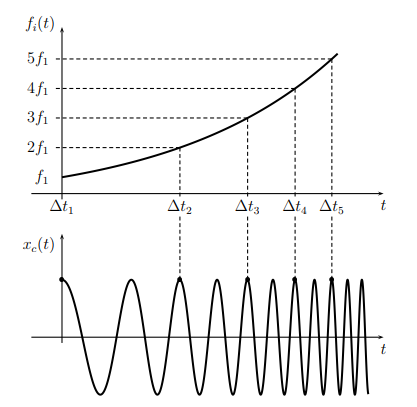
\includegraphics[width=0.5\linewidth]{figuras/SSS}
	\caption{Em cima: Frequência instantânea $f_{i}$. Embaixo: \textit{swept signal} sincronizado. Autor: \cite{novak2010chebyshev}}
	\label{fig:sss}
\end{figure}

\chapter{Metodologia} \label{cap3}

\section{Caracterização}

%\subsection*{Método de caracterização baseado na convolução não linear}
O método de caracterização foi baseado nos experimentos realizados por \cite{farina2001non} e utiliza o sinal de excitação de um sistema não linear descrito na subseção \ref{ident}. O método consiste em excitar o sistema em análise com um \textit{Swept Sine} e gravar a saída do sistema. Em seguida	realiza-se um inversão temporal do sinal de excitação que é utilizado para realizar uma convolução com a resposta gravada do sistema em análise. Após essa convolução, obtém-se uma função constituída por respostas ao impulso seguidas conforme a figura \ref{fig:nlcir}.

\begin{figure}[!htb]
	\centering
	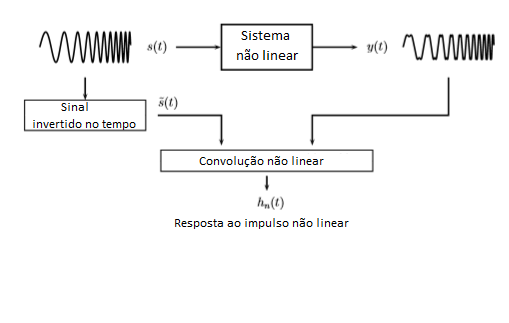
\includegraphics[width=0.9\linewidth]{figuras/NLCM}
	\caption{Diagrama de blocos do método baseado em convolução não linear. Autor: \cite{novakdissertation}}
	\label{fig:nlcm}
\end{figure}

A figura \ref{fig:nlcm} mostra os sinais $s(t)$ e $y(t)$ que são respectivamente, o sinal senoidal que varia exponencialmente na frequência e a saída do sistema em análise. O sinal $\overline{s}(t)$ é o sinal $s(t)$ invertido temporalmente. A convolução entre $y(t)$ e $\overline{s}(t)$ pode ser expressa por:
\begin{equation}
y(t) \ast \overline{s}(t) = \sum_{m=1}^{\infty}h_{m}(t + \Delta t_{m})
\label{kernel}
\end{equation}
Onde, $h_{m}$ é a resposta não linear ao impulso e $\Delta t_{m}$ é a diferença de tempo entre a primeira resposta impulsional e a m-ésima resposta do sistema, onde a primeira resposta define a parte linear do sistema em análise. Dessa forma é possível separar temporalmente cada resposta ao impulso, a partir do valor de $\Delta t_{m}$ como mostra a figura abaixo:

\begin{figure}
	\centering
	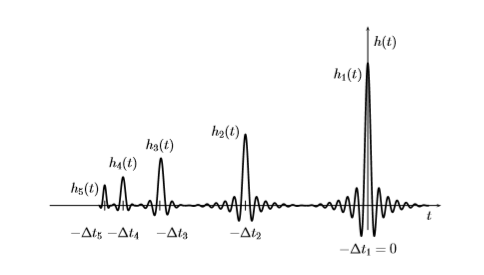
\includegraphics[width=0.6\linewidth]{figuras/NLCIR}
	\caption{Resposta ao impulso do sistema em análise. Autor: \cite{novakdissertation}}
	\label{fig:nlcir}
\end{figure}

Através do uso da Transformada de Fourier de cada resposta ao impulso é obtida a resposta frequencial de cada impulso como mostra a figura \ref{fig:nlcfr}
\begin{figure}
	\centering
	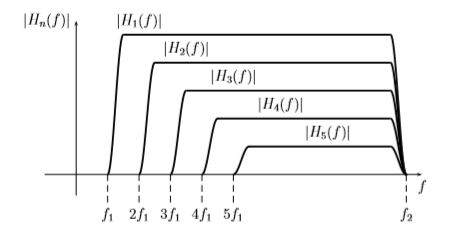
\includegraphics[width=0.6\linewidth]{figuras/NLCFR}
	\caption{Módulo da resposta frequencial dos impulsos. Autor:\cite{novakdissertation}}
	\label{fig:nlcfr}
\end{figure}

Na figura \ref{fig:nlcfr}, as frequências $f_{1}$ e $f_{2}$ são as frequências em que o sinal de excitação começa e termina, respectivamente.

\section{Metodologia utilizada para caracterizar um modelo}\label{Metodologia}

Utilizando o método de caracterização proposto por Farina em \cite{farina2001non} e por Novak em \cite{novak2010nonlinear}, que consiste em alimentar um sistema não linear com um sinal senoidal que varia a sua frequência de forma exponencial, criou-se um modelo de amplificador virtual com as características de um modelo físico.

O amplificador utilizado para a caracterização, mostrado na figura \ref{fig:Black}, é um \textit{Blackstar} HT-5 C, composto por uma válvula 12BH7 no pré amplificador e uma ECC83 na parte de amplificação de potência. Diferente da tentativa de caracterização realizada em trabalhos passados, a caracterização foi feita gravando a saída do pré amplificador, simplificando a quantidade de equipamentos utilizados, evitando ao máximo a captação de ruídos para tenta obter o sinal mais limpo de interferências possíveis.

\begin{figure}
	\centering
	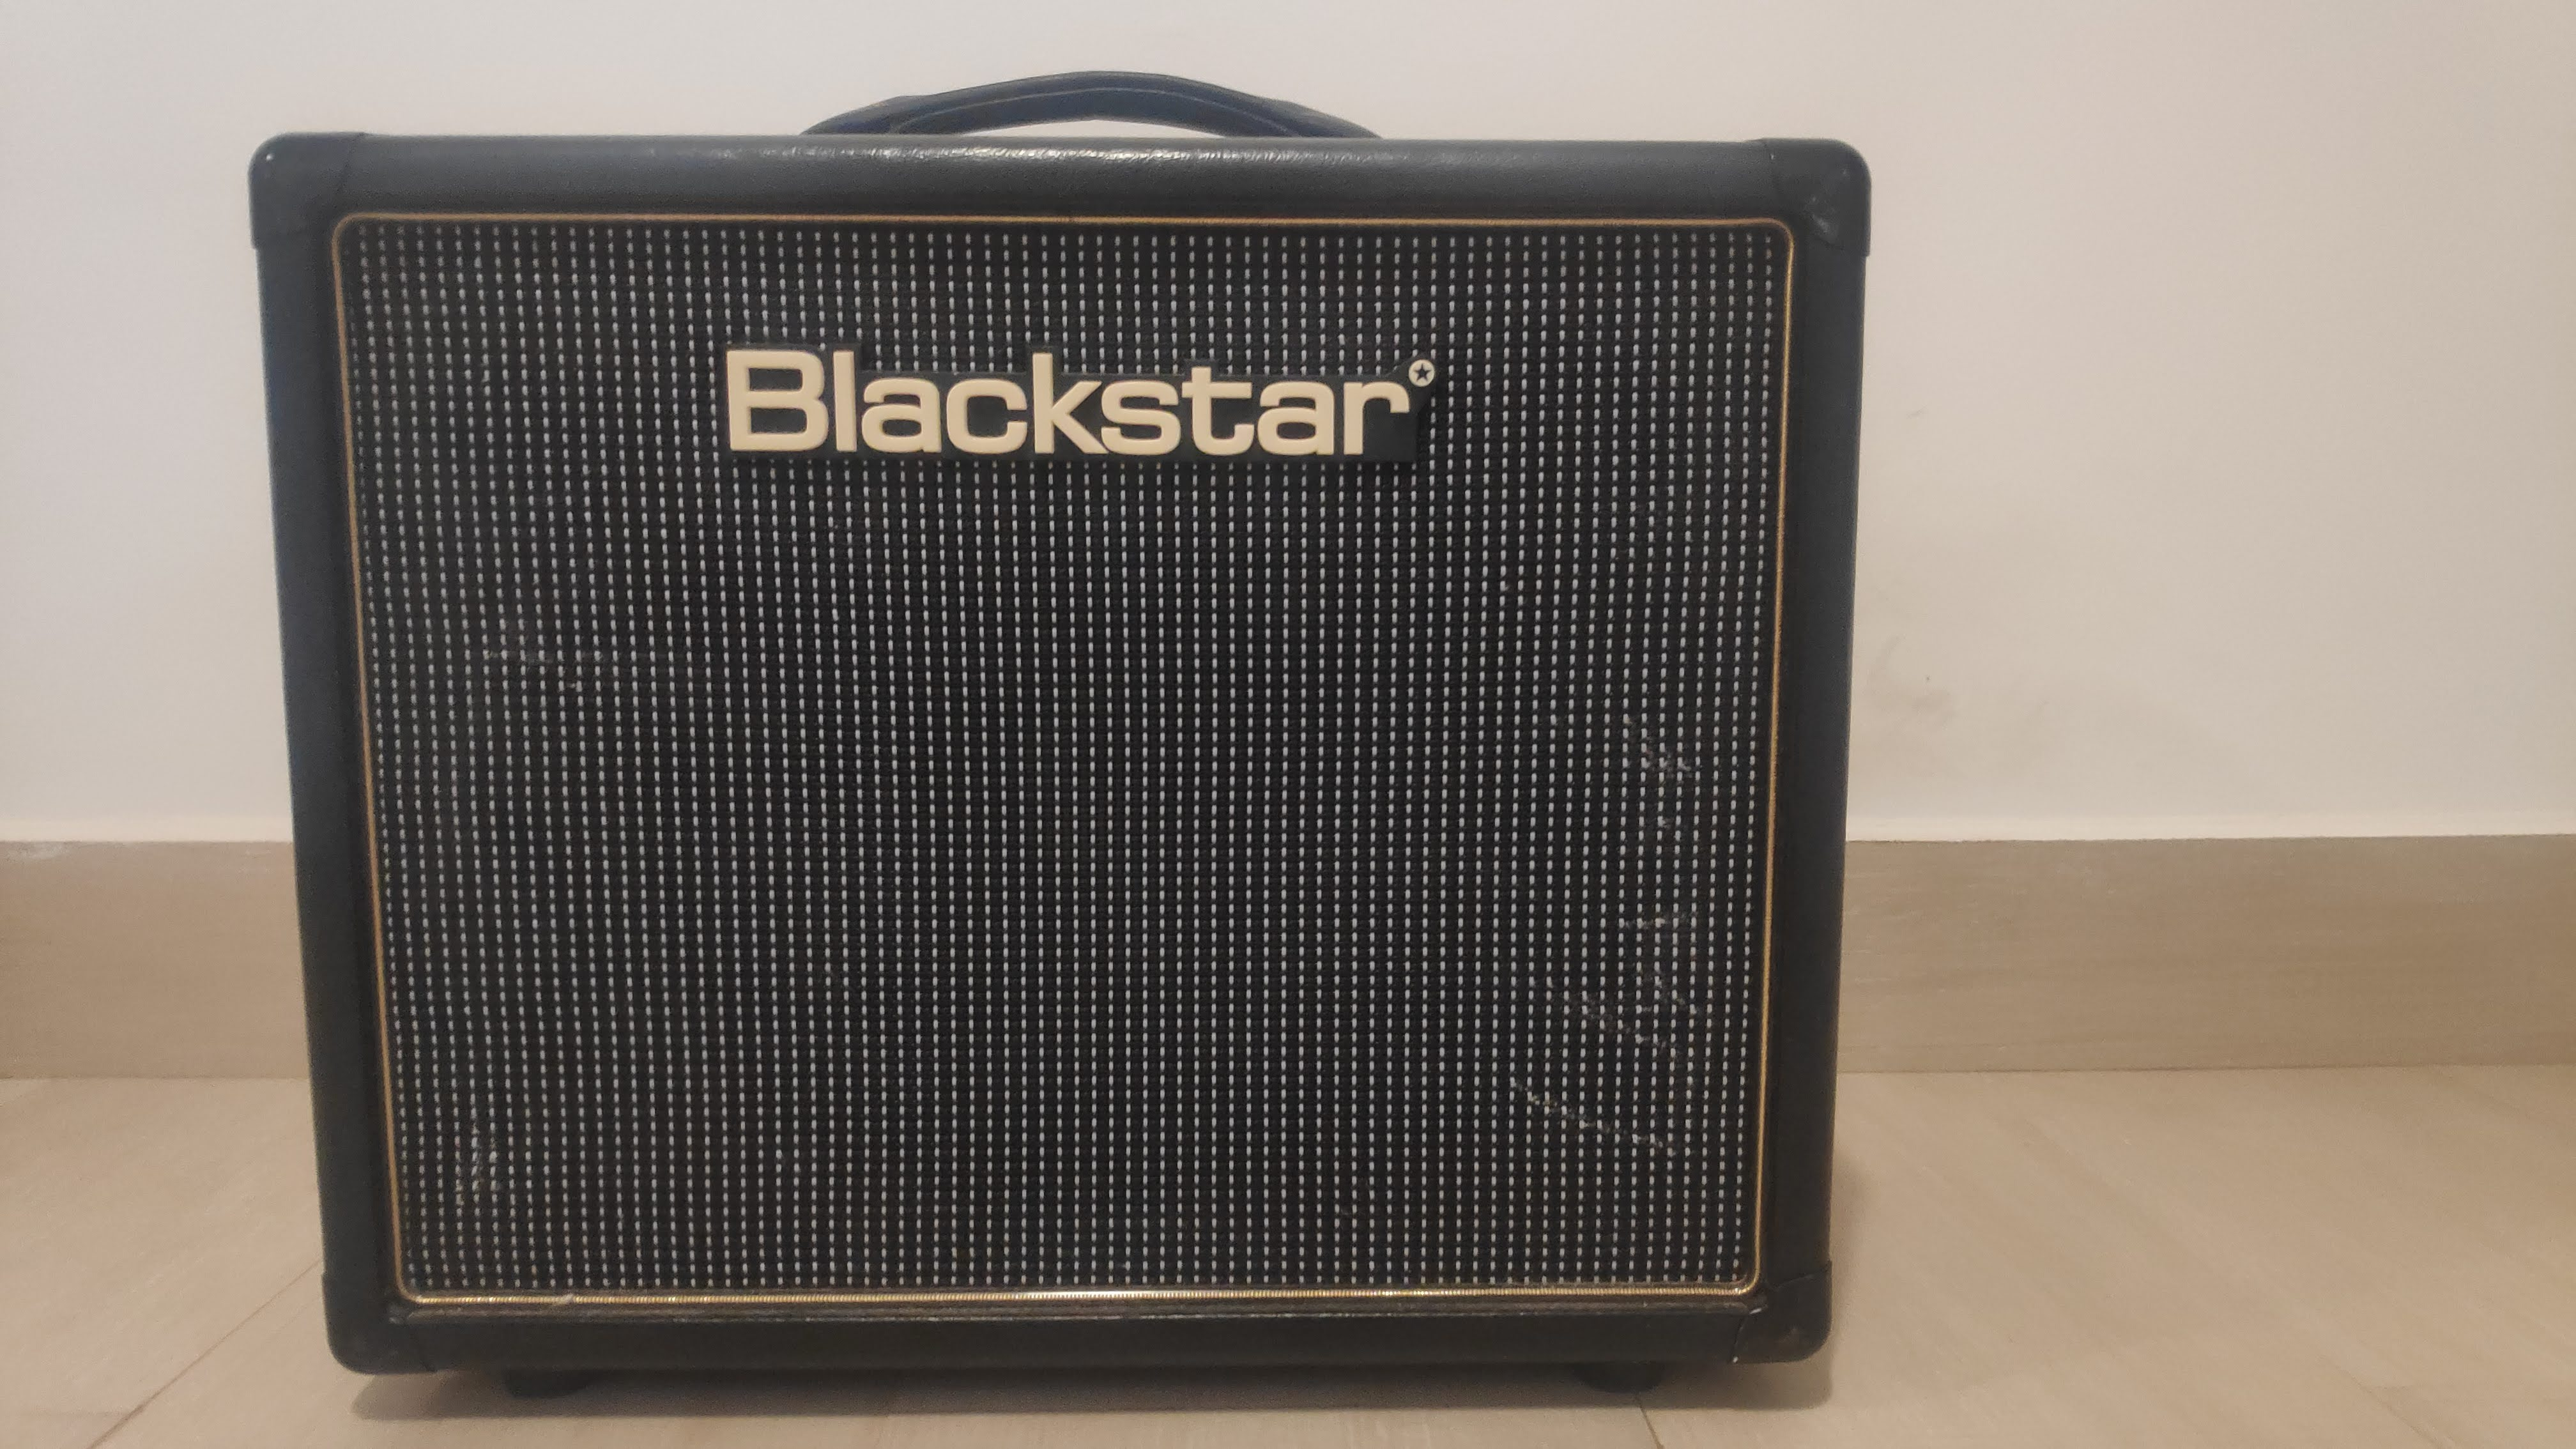
\includegraphics[width=0.5 \linewidth]{figuras/Blackstar1}
	\caption{Amplificador Blackstar HT-5 C}
	\label{fig:Black}
\end{figure}

A criação do sinal de teste foi feita segundo a equação \ref{sinal exponencial}, utilizando o programa Matlab para computar a função e gerar o arquivo de áudio em formato \textit{.wav}. O tempo de duração do sinal foi de 20 segundos, gerando 882000 amostras, devido a frequência de amostragem de 44,1 kHz que foi igualada a frequência da interface de áudio USB utilizada durante o processo de gravação dos sinais.


O sinal exponencial então foi exportado em uma trilha mono, para o programa Audacity, que é um editor, gravador e reprodutor de áudio e configurada para enviar o sinal para a saída da interface. Utilizando a interface de áudio M-audio \textit{Fast Track Pro}, conectou-se a saída do pré amplificador presente no \textit{Blackstar} à entrada de áudio da interface, através de um cabo P10. A saída da interface, por onde o sinal exponencial é enviado do computador, foi conectada à entrada de instrumentos do amplificador. No software Audacity, foi criada uma segunda trilha de áudio armada para gravar o sinal na entrada da interface. 


A figura \ref{fig:diag} mostra como foram feitas as conexões entre computador, interface e amplificador.
\begin{figure}
	\centering
	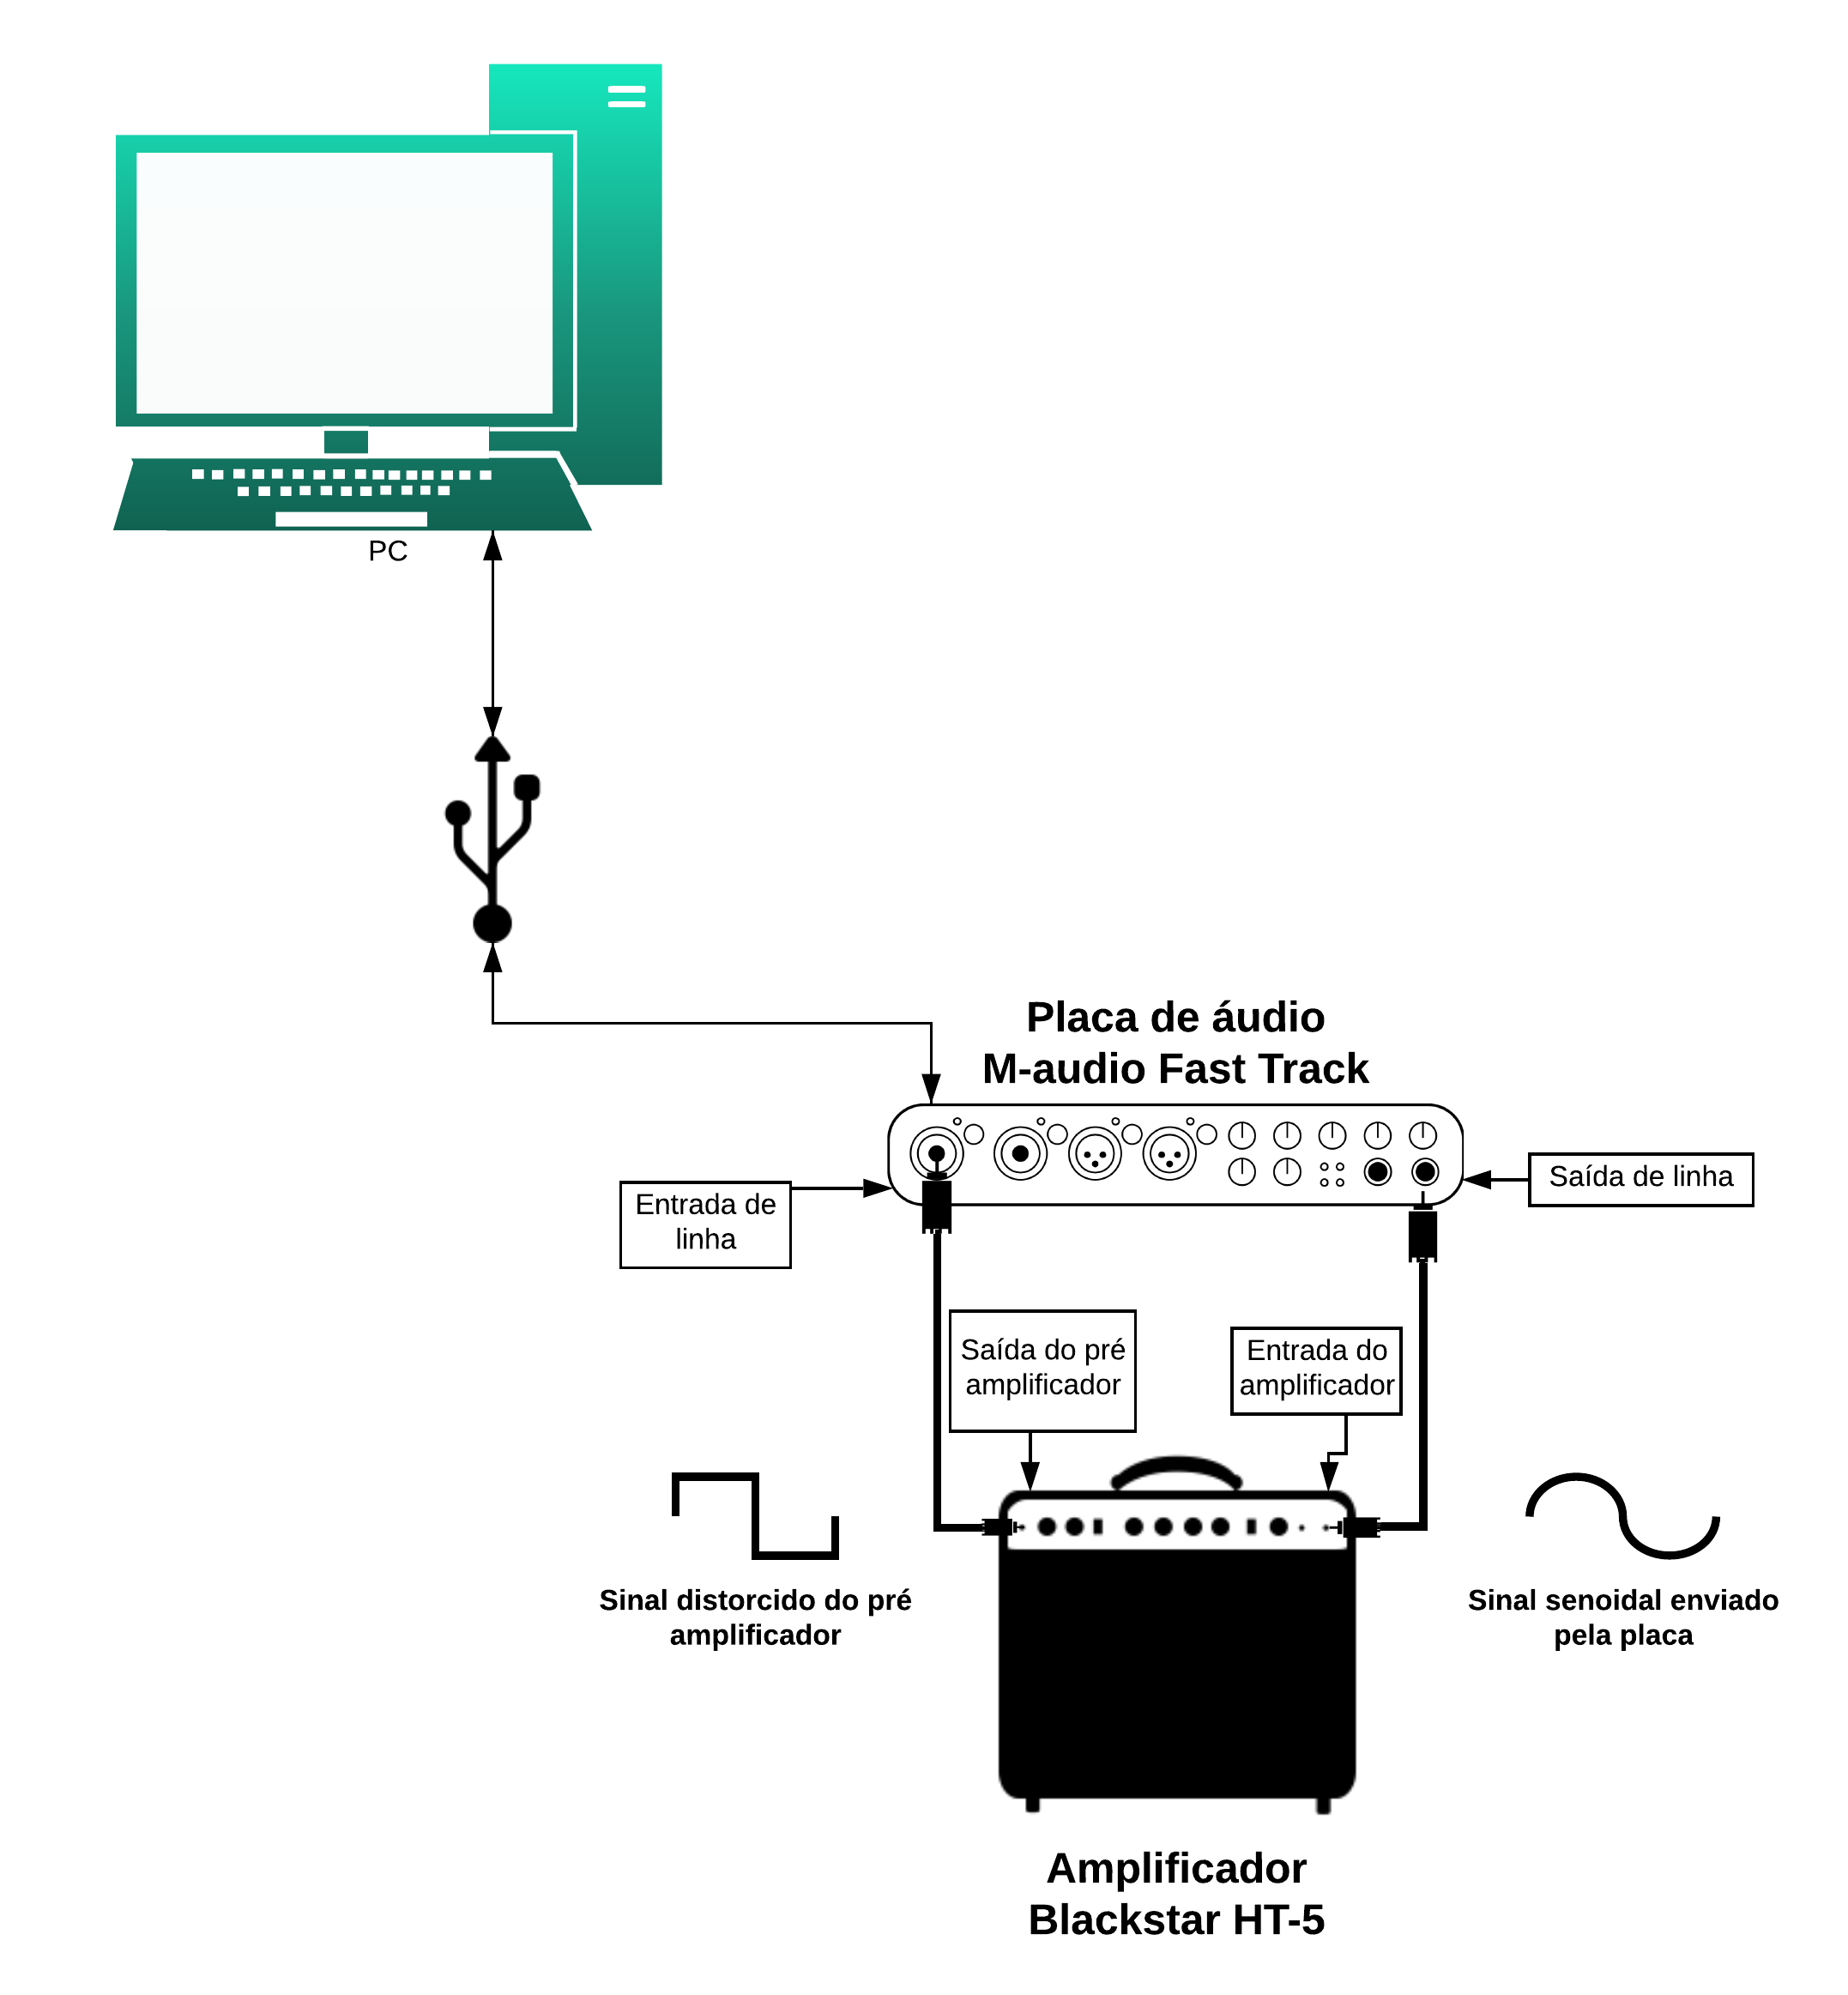
\includegraphics[width=0.7\linewidth]{figuras/diag}
	\caption{Diagrama de conexão do sistema de caracterização}
	\label{fig:diag}
\end{figure}

Após a gravação do sinal exponencial na saída do pré amplificador, o arquivo contendo as informações foi exportado para o Matlab onde foi processado e convoluído com o sinal exponencial invertido para obtenção dos \kernels, como mostra a figura \ref{fig:nlcm}. Seguindo a extração dos \kernels, separou-se cada impulso obtido para a construção do modelo de \textit{Hammerstein} do amplificador, exemplificado na figura \ref{fig:hammer}


\begin{figure}
	\centering
	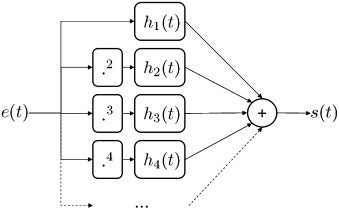
\includegraphics[width=0.5\linewidth]{figuras/hammer}
	\caption{Modelo de \textit{Hammerstein}. Retirado de: \cite{inproceedings}}
	\label{fig:hammer}
\end{figure}

\pagebreak
A ordem do sistema, ou seja, a quantidade de \kernels utilizados para construir o modelo de \textit{Hammerstein}, foi ajustada para utilizar 11 \kernels. A saída do sistema então foi obtida, com a convolução de 11 sinais, cada um elevado a um expoente, cujo valor máximo é determinado pela ordem do sistema, com o \kernels associado a cada expoente. Esses sinais são somados e resultando em um único sinal de áudio que representa a saída final do modelo caracterizado. A figura \ref{fig:diagramamatlab} exemplifica o funcionamento do algorítimo criado para a simulação do amplificador caracterizado.


\begin{figure}[!htb]

	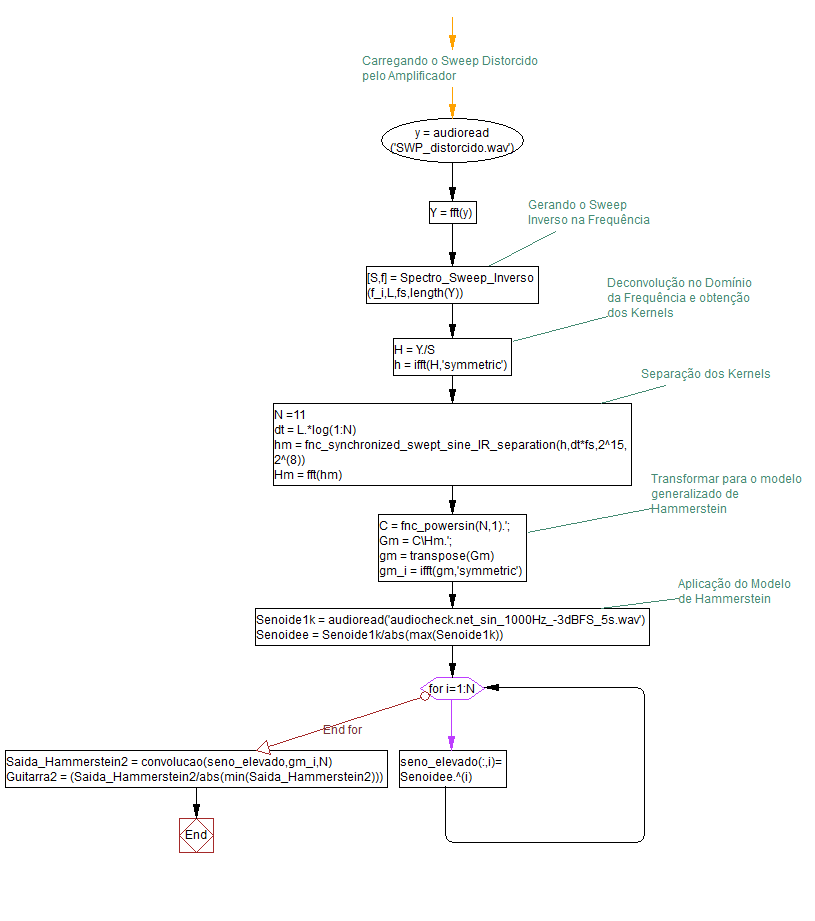
\includegraphics[width=1.0\linewidth]{figuras/Diagrama_Matlab}
	\caption{Fluxograma do programa desenvolvido}
	\label{fig:diagramamatlab}
\end{figure}

\chapter{Resultados}




A montagem do sistema de \textit{Hammerstein}, permitiu que fosse criada um modelo virtual do amplificador. Para verificar o funcionamento e performance do sistema criado, foi utilizado um único sinal de entrada para o amplificador real e o modelo virtual. O sinal de teste aplicado foi uma senoide de 1 kHz, mostrada na figura \ref{fig:tccfig}, na parte superior da imagem. Na parte inferior da figura \ref{fig:tccfig}, em azul está plotado a saída gravada do amplificador físico, em laranja, sobrepondo quase que por completo a cor azul, é a saída do modelo virtual do amplificador.

\begin{figure}
	\centering
	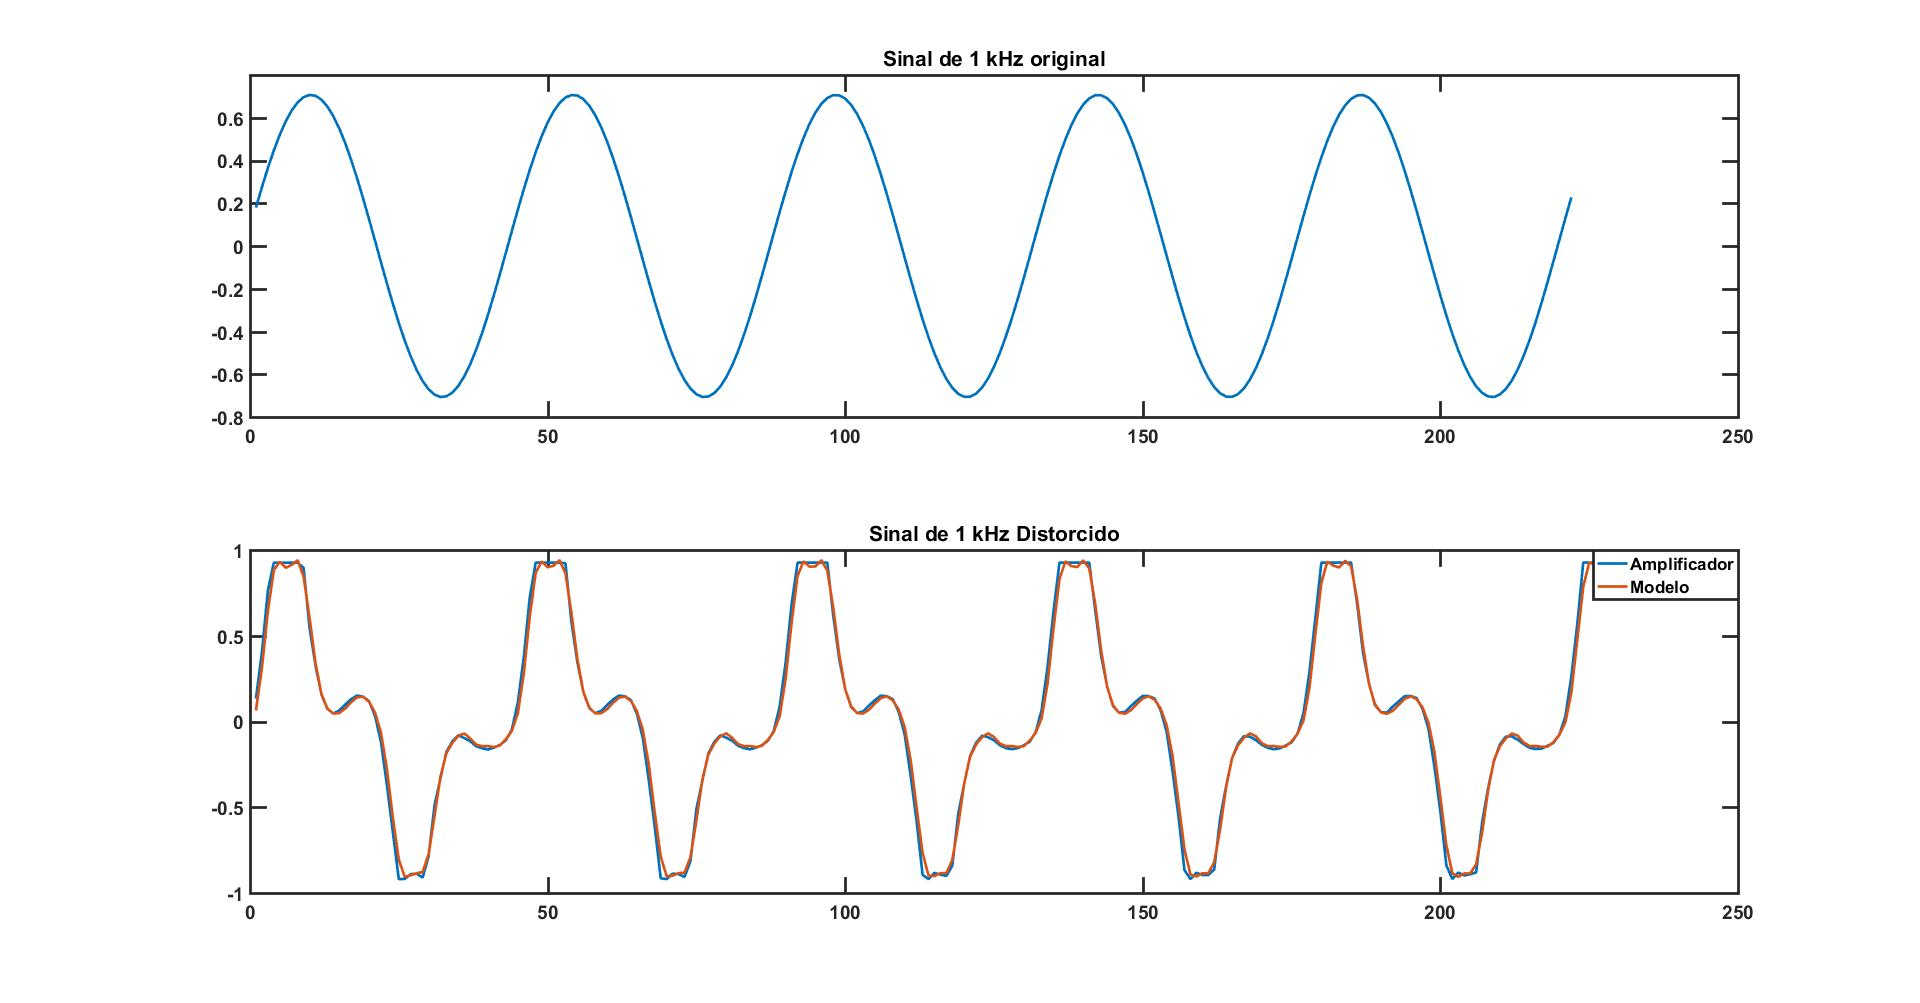
\includegraphics[width=1\linewidth]{figuras/TCC_fig}
	\caption{Superior: Sinal senoidal de 1 kHz utilizado para testar os modelos. Inferior: Em azul está o sinal distorcido pelo amplificador físico, em laranja a saída do modelo de \textit{Hammerstein}}
	\label{fig:tccfig}
\end{figure}

Para medir valores mais concretos entre as saídas gravadas do modelo real e físico, foi aplicado aos sinais gravados de cada modelo, a Transformada de Fourier para visualizar a resposta em frequência dos amplificadores. Na figura \ref{fig:tcc2fft}, na parte superior é mostrada a resposta frequencial do amplificador físico, já na parte inferior, a resposta frequencial do modelo. Através desse tipo de análise, é possível ter uma ideia das diferenças de intensidade entre os harmônicos gerados pelo modelo físico e pelo modelo de \textit{Hammerstein}. A tabela \ref{tab01}, mostra as medidas realizadas para cada harmônico entre os modelos, como se trata de um valor de intensidade de som, a unidade utilizada para os valores está de \textit{decibels}.
\begin{table}[h]
	\centering
	\caption{Propriedades obtidades após processamento}
	\label{tab01}
	
	\begin{tabular}{ccccc}
		\toprule
		\textbf{Harmônico} & \textbf{Amplificador (dB)} & \textbf{Modelo(dB)} & \textbf{Diferença (dB)} & \textbf{\% erro}  \\
		\midrule
		Fundamental & 48,20 & 48,36 & -0,16 & 0\% \\
		2º & 39,06 & 38,99 & 0,06 & 0\%  \\
		3º & 16,1 & 45,67 & 0,43 & 1\% 	\\
		4º & 37,09 & 37,65 & -0,56 & -2\% \\
		5º & 33,45 & 34,60 & -1,15 & -3\% \\ 
		6º & 33,73 & 31,84 & 1,89 & 6\%   \\ 
		7º & 36,68 & 36,42 & 0,26 & 1\%   \\ 
		8º & 35,49 & 34,22 & 1,27 & 4\%   \\ 
		9º & 35,90 & 34,84 & 1,06 & 3\%   \\ 
		10º & 32,44 & 32,06 & 0,37 & 1\%  \\ 
		11º & 32,07 & 30,67 & 1,39 & 4\%  \\
		\bottomrule
	\end{tabular}
	\label{Resultados obtidos}
	\caption{Resultados obtidos}
\end{table}

Os dados das tabelas mostram pequenas divergências entre os modelos, como no sexto harmônico, onde foi obtido o maior erro entre todos. Alguns harmônicos, como no caso do Fundamental e de outros, ultrapassa o valor do harmônico produzido pelo amplificador real. Por se tratar de uma digitalização, passando de um meio físico para um meio virtual, pela utilização de cabos e conectores e de uma interface de áudio, que realiza uma amostragem do sinal através de um conversor analógico digital, é de extrema dificuldade criar um modelo fiel, que consiga modificar o som de modo idêntico ao amplificador real, porém esse modelo pode alcançar resultados próximos o suficiente, possibilitando o uso de modelos desenvolvidos através dessa técnica.



\begin{figure}[!htb]
	\centering
	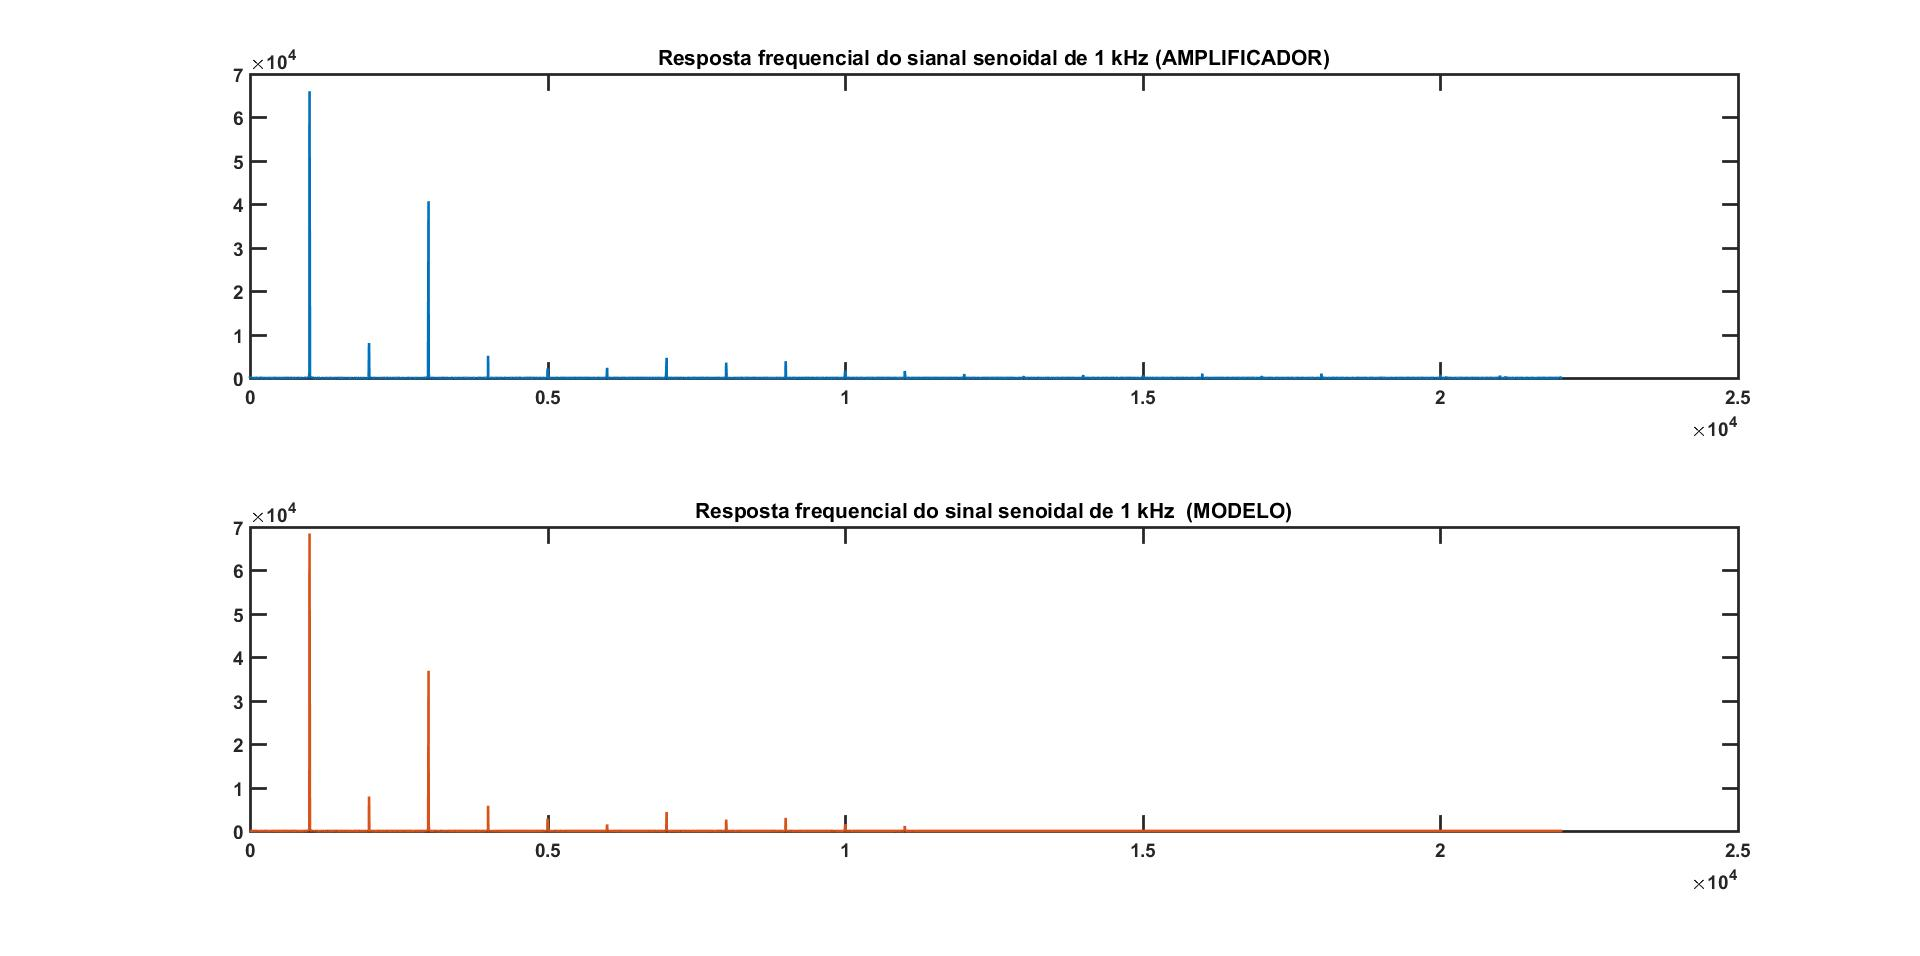
\includegraphics[width=1\linewidth]{figuras/Resp_freq}
	\caption{Resposta em frequência dos modelos}
	\label{fig:tcc2fft}
\end{figure}
Além de todos os equipamentos, cabos e conectores utilizados para a gravação dos sinais, existe uma relação máxima entre a ordem do modelo e a viabilidade de separação dos \kernels. O primeiro \textit{kernel}, observado bem no centro da figura \ref{fig:10sweepkernels} é separado por uma distância razoável do segundo \textit{kernel}, mas com o passar dos \kernels essa distância diminui, assim como suas intensidades, podendo ser considerado apenas ruído. A separação entre eles é dada pela equação \ref{kernel}, onde o $\Delta t_{m}$ é definido por:
\begin{equation}
\Delta t_{m} =  L \ln(m),
\label{eq:Delta_t_m}
\end{equation}

O parâmetro L na equação \ref{eq:Delta_t_m} é definido pelos parâmetros iniciais do sinal de excitação do sistema durante a caracterização e pode ser calculado através da equação \ref{Equação 5.10}
\begin{figure}
	\centering
	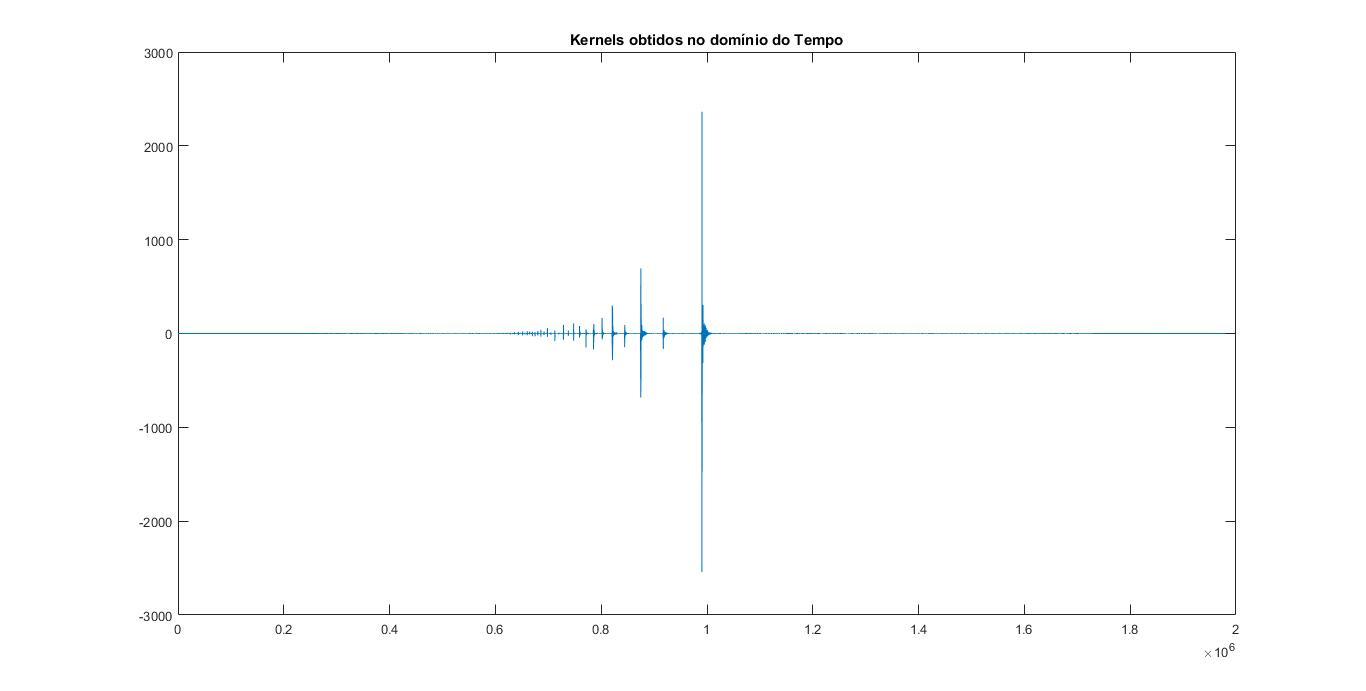
\includegraphics[width=0.7\linewidth]{figuras/10Sweep_Kernels}
	\caption{\kernels obtidos}
	\label{fig:10sweepkernels}
\end{figure}

Além da intensidade dos \kernels diminuir, eles tendem a estreitar os espaços, dificultando a separação de cada \textit{kernel} com a utilização de sistemas que utilizam ordens elevadas.

\chapter{Conclusão}


%%\chapter[Elementos do Pós-Texto]{Elementos do Pós-Texto}

Este capitulo apresenta instruções gerais sobre a elaboração e formatação dos 
elementos do pós-texto a serem apresentados em relatórios de Projeto de 
Graduação. São abordados aspectos relacionados a redação de referências 
bibliográficas, bibliografia, anexos e contra-capa.

\section{Referências Bibliográficas}

O primeiro elemento do pós-texto, inserido numa nova página, logo após o último 
capítulo do trabalho, consiste da lista das referencias bibliográficas citadas 
ao longo do texto.

Cada referência na lista deve ser justificada entre margens e redigida no 
formato Times New Roman com 11pts. Não é necessário introduzir uma linha em 
branco entre referências sucessivas.

A primeira linha de cada referencia deve ser alinhada a esquerda, com as demais 
linhas da referencia deslocadas de 0,5 cm a partir da margem esquerda. 

Todas as referências aparecendo na lista da seção \lq\lq Referências 
Bibliográficas\rq\rq\ devem estar citadas no texto. Da mesma forma o autor deve 
verificar que não há no corpo do texto citação a referências que por 
esquecimento não forma incluídas nesta seção.

As referências devem ser listadas em ordem alfabética, de acordo com o último 
nome do primeiro autor. Alguns exemplos de listagem de referencias são 
apresentados no Anexo I.

Artigos que ainda não tenham sido publicados, mesmo que tenham sido submetidos 
para publicação, não deverão ser citados. Artigos ainda não publicados mas que 
já tenham sido aceitos para publicação devem ser citados como \lq\lq in 
press\rq\rq.

A norma \cite{NBR6034:2000}, que regulamenta toda a formatação a ser usada na 
elaboração de referências a diferente tipos de fontes de consulta, deve ser 
rigidamente observada. Sugere-se a consulta do trabalho realizado por 
\cite{arruda2007}, disponível na internet.

\section{Anexos}

As informações citadas ao longo do texto como \lq\lq Anexos\rq\rq\ devem ser 
apresentadas numa seção isolada ao término do trabalho, após a seção de 
referências bibliográficas. Os anexos devem ser numerados seqüencialmente em 
algarismos romanos maiúsculos (I, II, III, ...). A primeira página dos anexos 
deve apresentar um índice conforme modelo apresentado no Anexo I, descrevendo 
cada anexo e a página inicial do mesmo.

A referência explícita no texto à um dado anexo deve ser feita como 
\lq\lq Anexo 1\rq\rq. Referências implícitas a um dado anexo devem ser feitas 
entre parênteses como (Anexo I). Para referências a mais de um anexo as mesmas 
regras devem ser aplicadas usando-se o plural adequadamente. Exemplos:
\begin{itemize}
	\item \lq\lq Os resultados detalhados dos ensaios experimentais são 
	apresentados no Anexo IV, onde ...\rq\rq

	\item \lq\lq O Anexo I apresenta os resultados obtidos, onde pode-se 
	observar que ...\rq\rq

	\item \lq\lq Os Anexos I a IV apresentam os resultados obtidos ...\rq\rq

	\item \lq\lq Verificou-se uma forte dependência entre as variáveis citadas 
	(Anexo V), comprovando ...\rq\rq
\end{itemize}



\bookmarksetup{startatroot} 

\postextual

\bibliography{bibliografia} 
%\begin{apendicesenv}

\partapendices

\chapter{Primeiro Apêndice}

Texto do primeiro apêndice.

\chapter{Segundo Apêndice}

Texto do segundo apêndice.

\end{apendicesenv}

%\begin{anexosenv}

\partanexos

\chapter{Primeiro Anexo}

Texto do primeiro anexo.

\chapter{Segundo Anexo}

Texto do segundo anexo.

\end{anexosenv}


\printindex

\end{document}

